
%%%%%%%%%%%%%%%%%%%%%%%%%%%%%%%%%%%%%%%%%%%%%%%%%%%%%%%%%%%%%%%%%%%%%%%%%%%
%DO NOT MAKE CHANGES IN THIS FILE

\documentclass[12pt, a4paper]{report}
\usepackage[left = 1.5in, right = 1in, top = 1in, bottom = 1in]{geometry}%for margin
\usepackage{amsfonts, amsmath, amssymb} %for mathematical equations
\usepackage{graphicx} %for images

\usepackage{times} %font Times New Roman Font
\usepackage{float} %required if you use H(strictly here) position for floats
\usepackage[skip = 8pt,tableposition=top, figureposition=bottom]{caption}%adjust spacing of captions and specify where captions are
\usepackage{hyperref} % for easy Navigation in document, also puts links in TOC, LOF, LOT...
\usepackage{setspace} %to change line spacing in some portion \singlespacing \onehalfspacing \doublespacing
\usepackage{acro} %for List of Abbrreviation and Symbol
\acsetup{first-style = short} % set to display only short form on the command \ac{}

%packages required for complex tables
\usepackage{bigstrut} 
\usepackage{multirow}
%package for greek letters
\usepackage[euler]{textgreek}
\renewcommand{\contentsname}{Table of Contents} %Change TOC Heading ... default is "Contents" 

\parindent 0pt	%removes the indent in paragraph
\setlength{\parskip}{18pt}	%for paragraph spacing
\renewcommand{\baselinestretch}{1.5}   %Line Spacing = 1.5 line-spaces

%to reduce spacing in sections
\usepackage{titlesec}
\titlespacing*{\section}{0pt}{0pt}{0pt} %left, top, bottom spacings
\titlespacing*{\subsection}{0pt}{0pt}{0pt}
\titlespacing*{\subsubsection}{0pt}{0pt}{0pt}
\titlespacing*{\paragraph}{0pt}{0pt}{0pt}
\titlespacing*{\subparagraph}{0pt}{0pt}{0pt}

%adjust fontsizes\ of sections
\titleformat*{\section}{\fontsize{14pt}{18pt}\bfseries}
\titleformat*{\subsection}{\fontsize{13pt}{18pt}\bfseries}
\titleformat*{\subsubsection}{\fontsize{12pt}{18pt}\bfseries}
\titleformat*{\paragraph}{\fontsize{12pt}{18pt}\bfseries}
\titleformat*{\subparagraph}{\fontsize{12pt}{18pt}\bfseries}

%to reduce separation between points in list
\usepackage{enumitem}
\setlist[enumerate]{nosep} % no separation between items in enumerate
\setlist[itemize]{nosep} % no separation between items in itemize
%use \vspace{-18pt} before list to reduce paragraph spacing between list and preceeding paragraph.

%Changes for Chapter Heading Spacing and formats for numbered chapters
\makeatletter
\def\@makechapterhead#1{%
  %\vspace*{50pt}%
  {  \MakeUppercase{\ifnum \c@secnumdepth >\m@ne
        \fontsize{16pt}{1}\bfseries \@chapapp \space \thechapter\vspace{5pt}\\
    \fi
    \interlinepenalty\@M
     \bfseries #1}\par\nobreak
    %\vskip 0pt
  }}
\makeatother

%%%%%%%%%%%%%%%%%%%%%%%%%%%%%%%%%%%%%%%%%%%%%%%%%%%%%%%%%%%
%to adjust Heading spacings and fonts For unnumbered chapters, TOC, LOF ...
\makeatletter
% Redefine the \chapter* header macro to remove vertical space
\def\@makeschapterhead#1{%
  %\vspace*{50\p@}% Remove the vertical space
  {\newpage \parindent \z@ \raggedright
    \normalfont
    \interlinepenalty\@M
    \center \fontsize{16pt}{1} \bfseries \MakeUppercase{#1}\par\nobreak
    %\vskip 18\p@ % adjust space after heading 18pt
  }}
\makeatother 
%%%%%%%%%%%%%%%%%%%%%%%%%%%%%%%%%%%%%%%%%%%%%%%%%%%%%%%%%%%

%%%%%%%%%%%%%%%%%%%%%%%%%%%%%%%%%%%%%%%%%%%%%%%%%%%%%%%%%%%%%%%%%%%%%%%%%%%
% newcommand for generating Cover Page
\newcommand{\KECcoverpage}
{
\begin{titlepage}
\begin{center}
\Large{\textbf{KANTIPUR ENGINEERING COLLEGE}}\\
\large{\textbf{(Affiliated to Tribhuvan University)}}\\
\large{\textbf{Dhapakhel, Lalitpur}}\\
\vfill	%vertically fill the space 
\begin{figure}[h] % h: put logo "here"
\begin{center}

\includegraphics[width=25mm, height = 25mm]{images/logo.png}
\end{center}
\end{figure}

\large{\textbf{[Subject Code: \subCode]}}\\ %Chcite handeu ta iza}ange This Line
\large{\textbf{A \MakeUppercase{\project} \MakeUppercase{\doc} ON}}\\ %Change This Line
\Large{\textbf{\MakeUppercase{\projectTitle}}}\\

\vfill	%vertically fill the space 
\large{\textbf{Submitted by:}}\\
\large{\textbf{\submittedBy}}\\
\vfill	%vertically fill the space 
\textbf{A \MakeUppercase{\project} SUBMITTED IN PARTIAL FULFILLMENT OF THE REQUIREMENT FOR THE DEGREE OF \MakeUppercase{\degree}}\\

\vfill	%vertically fill the space 
\large{\textbf{Submitted to:}}\\
\large{\textbf{\submittedTo}}\\
\vfill
\large{\textbf{\defDay\ \defMonth, \defYear}}
\pagebreak
\end{center}
\end{titlepage}
}
%%%%%%%%%%%%%%%%%%%%%%%%%%%%%%%%%%%%%%%%%%%%%%%%%%%%%%%%%%%%%%%%%%%%%%%
% newcommand for generating Cover Page
%Title Page
\newcommand{\KECtitlepage}
{
\begin{titlepage}
\begin{center}
\Large{\textbf{\MakeUppercase{\projectTitle}}}\\

\vfill	%vertically fill the space 

\large{\textbf{Submitted by:}}\\
\large{\textbf{\submittedBy}}\\

\if{\ne{\supervisor}{none}} \\ Displays Supervisor name only if it is not "none"
	\vfill	%vertically fill the space 
	\large{\textbf{Supervised by:}}\\
	\large{\textbf{\supervisor}}\\
	\large{\textbf{\degSup}}\\
\fi
\vfill	%vertically fill the space 
\textbf{A \MakeUppercase{\project} SUBMITTED IN PARTIAL FULFILLMENT OF THE REQUIREMENT FOR THE DEGREE OF \MakeUppercase{\degree}}\\

\vfill	%vertically fill the space 
\large{\textbf{Submitted to:}}\\
\large{\textbf{\submittedTo}}\\
\large{\textbf{Kantipur Engineering College}}\\
\large{\textbf{Dhapakhel, Lalitpur}}\\

\vfill
\large{\textbf{\defDay\ \defMonth, \defYear}}
\thispagestyle{empty}\\ %to remove page number
\pagebreak
\end{center}
\end{titlepage}
}
%%%%%%%%%%%%%%%%%%%%%%%%%%%%%%%%%%%%%%%%%%%%%%%%%%%%%%%%%%%%%%%%%%%%%%
%command for copyright page
\newcommand{\KECcopyright}
{
\chapter*{Copyright}%Required only for Final Defense of Major Project
\addcontentsline{toc}{chapter}{Copyright}
The author has agreed that the library, Kantipur Engineering Collage, may make this report freely available for inspection. Moreover the author has agreed that permission for extensive copying of this report for scholarly purpose may be granted by the supervisor(s), who supervised the project work recorded herein or, in their absence, by the Head of the Department wherein this project was done. It is understood that due recognition will be given to the author of this report and to the \submittedTo, Kantipur Engineering College in any use of the material of this report. Copying or publication or other use of this report for financial gain without approval of the \submittedTo, Kantipur Engineering College and author’s written permission is prohibited.\par Request for permission to copy or to make any other use of the material in this report in whole or in part should be addressed to:

Head\\
\submittedTo\\
Kantipur Engineering College\\
Dhapakhel, Lalitpur\\
Nepal
}
%%%%%%%%%%%%%%%%%%%%%%%%%%%%%%%%%%%%%%%%%%%%%%%%%%%%%%%%%%%%%%%%%%%%%%
%command for Approval Letter
\newcommand{\KECapproval}
{
\chapter*{Kantipur Engineering College
\vskip -10pt}%Required only for Final Defense of Major Project
\begin{center}
\fontsize{12.8pt}{1} %size decreaced to adjust department name in single line
\textbf{
\MakeUppercase{\submittedTo}\\ %for department name
}
\vskip 10pt
\fontsize{16pt}{1}
\textbf{APPROVAL LETTER}
\end{center}
\vskip -16pt
\addcontentsline{toc}{chapter}{Approval Letter}%
The undersigned certify that they have read and recommended to the Institute of Engineering for acceptance, a project report entitled "\projectTitle " submitted by \\
\submittedBy \\
in partial fulfillment for the degree of \degree. \par
{\vspace{25pt}
..........................................\\
Supervisor\\
\supervisor \\
\degSup\\
\vspace{25pt}\\
..........................................\\
External Examiner\\
\external\\
\degExternal\\
\vspace{25pt}\\
..........................................\\
\hod\\
Head of Department\\
\submittedTo
\vspace{10pt}\\
Date: \defMonth\space\defDay ,\space \defYear
\singlespacing\par
} %single spacing for the texts inside {}
}

%command for list of abbreviations
\newcommand{\KECloa}
{
%\chapter*{List of Abbreviations}
\addcontentsline{toc}{chapter}{List of Abbreviations}
\vskip -42pt % to reduce space due to invisivle acronym class name
{
\singlespacing
\printacronyms[include-classes=abbr, name= List of Abbreviations ]
}

}

%command for list of symbols
\newcommand{\KEClos}
{
\chapter*{List of Symbols}
\addcontentsline{toc}{chapter}{List of Symbols}
\vskip -42pt % to reduce space due to invisivle acronym class name{
{
\singlespacing
}
}

%command to adjust toc, lof, lot spacing
\newcommand{\KECadjusttocspacings}
{
\parskip 0pt % to remove paragraph spacing in TOC, LOF ...
\renewcommand{\baselinestretch}{0.1} % to adjust line spacing in toc
\newcommand*{\noaddvspace}{\renewcommand*{\addvspace}[1]{}}
\addtocontents{lof}{\protect\noaddvspace} %remove extra vertical space in LOF
\addtocontents{lot}{\protect\noaddvspace} %remove extra vertical space in LOT
}

 %includes the file KecReportFormat.tex that include all  necessary formattings
\usepackage{amsmath}
\usepackage{algorithm}
\usepackage{algorithmic}
%%%%%%%%%%%%%%%%%%%%%%%%%%%%%%%%%%%%%%%%%%%%%%%%%%%%%%%%%%%%%%%%%%%%%%%%%%%
%Define Macros for Details of your Project
\newcommand{\project}{Major Project } %Specify "Major Project" or "Minor Project"
\newcommand{\projectTitle}{FEATHERFIND : BIRD SPECIES IDENTIFICATION FROM AUDIO} %specify "Title" of Your Project
\newcommand{\doc}{Mid-Term Report} % specify the document you are preparing eg. "Proposal", "Mid-Term Report" or "Final Report"32
% Note that You have to sibmit "Final Report" for Pre-final defense as well.
\newcommand{\subCode}{CT707} %specify Subject of Your Project
\newcommand{\degree}{Bachelor in Computer Engineering}
%specify your degree
\newcommand{\submittedBy}%Specify Names and Roll/Symbol Numbers of the Project Group Members
{
    %Edit Member Names and Roll/Symbol No. and adjust width (\makebox[width]) if necessary 
    \makebox[9.9cm]{Gaurav Giri \hfill [Kan077bct034]}\\
    \makebox[10cm]{Iza K.C. \hfill [Kan077bct039]}\\
    \makebox[10cm]{Prajwal Khatiwada \hfill [Kan077bct056]}\\
    \makebox[10cm]{Samrat Kumar Adhikari \hfill [Kan077bct074]}\\

    %\makebox[9cm]{Member Name \hfill [Roll/Symbol No.]}\\
} % Note that You must write your "Symbol Numbers"(Exam Roll Numbers) for Final Defenses

\newcommand{\submittedTo}{Department of Computer and Electronics Engineering}
%specify your department
\newcommand{\hod}{Er. Rabindra Khati \\ Associate Professor}
%specify Head ot the department
\newcommand{\defYear}{2024} %Defense Year
\newcommand{\defMonth}{December} %Defense Month- January, February, ...
% \newcommand{\defDay}{22} %

\newcommand{\supervisor}{Prof. Dr. Subarna Shakya}
\newcommand{\degSup}{Project Coordinator\\ Department of Computer and
    Electronics Engineering}
\newcommand{\external}{External's Name}
\newcommand{\degExternal}{Designation of External\\Second line if required}
%Specify Name of External for Major Project (Required for Black Book) , use multiple lines (\\) if necessary

%%%%%%%%%%%%%%%%%%%%%%%%%%%%%%%%%%%%%%%%%%%%%%%%%%%%%%%%%%%%%%%%%%%%%%%%%%%

%%%%%%%%%%%%%%%%%%%%%%%%%%%%%%%%%%%%%%%%%%%%%%%%%%%%%%%%%%%%%%%%%%%%%%%%%%%
%Define Abberviations and Symbols
% NOTE that Only those Abberviations and Symbols that are included in document(using command \ac{}) will be displayed in the List of Abberviations and Symbols.

%class 'abbr': for List of Abbreviations

%%%%%%%%%%%%%%%%%%%%%%%%%%%%%%%%%%%%%%%%%%%%%%%%%%%%%%%%%%%%%%%%%
% class `symbol': for List of Symbols
%\DeclareAcronym{transparencyFactor}{
%  short = \ensuremath{\alpha} ,
% long  = Transparency Factor ,
% sort  = Transparency Factor , % string to compare for sorting symbols... default string is the acronym name -"transparencyFactor"
%class = symbol
%}% declares acronym named "transparencyFactor". Use \ac{UN} for short and \acl{UN} for long form.

%\DeclareAcronym{areaOfTriangle}{
% short = \ensuremath{a} , % use \ensuremath{a} instead of $a$
%% long  = Area of Triangle ,
% sort  = Area of Triangle , % string to compare for sorting symbols
%class = symbol
%}
%%%%%%%%%%%%%%%%%%%%%%%%%%%%%%%%%%%%%%%%%%%%%%%%%%%%%%%%%%%%%%%%%%%%%%%%%%%%%%%%%%%%%%%%%%%%%%%%%%%%
\setcounter{secnumdepth}{3}
%The Document
\begin{document}

\KECcoverpage
\KECtitlepage

\pagenumbering{roman}
%\KECapproval
% \chapter*{Acknowledgment}
% \addcontentsline{toc}{chapter}{Acknowledgment}%to include this chapter in TOC
% We would like to express our gratitude to everyone who helped us to complete this project.
% First and foremost, we would like to acknowledge the crucial role of our teachers of Department of Electronics and Computer Engineering for their guidance, support, and feedback throughout the project. Next, we would like
% to give our gratitude to our classmates, for providing constructive feedback and engaging in
% thought-provoking discussions regarding our project. Next, we’d like to thank all lecturers
% of our department for guiding us through the beginning of our project to the end. Finally,
% a special gratitude to our family and friends, for their love, encouragement, and support
% throughout our academic journey.\\
% Thank you all for your invaluable contributions to this project.\\
% \makebox[10cm]{Ajaya Chaudhary \hfill }\\
% \makebox[10cm]{Gaurav Giri \hfill }\\
% \makebox[10cm]{Iza K.C. \hfill }\\
% \makebox[10cm]{Lakesh Shrestha \hfill }
%to display members name under Acknowledgement
\chapter*{Abstract}
\addcontentsline{toc}{chapter}{Abstract}%to include this chapter in TOC 
% This report presents "FeatherFind", a comprehensive model designed for identifying bird species using audio recordings. The audio identification process involves collecting and preprocessing bird sound datasets, isolating key features using Mel Spectrogram, and employing EfficientNet, a state-of-the-art convolutional neural network, to accurately recognize bird calls.


    % {\textit{Keywords$-$Optical Character Recognition, Binarization, Thresholding, Denoising, Boundary Detection, Hough Line Transformation, K-Means Clustering, Convolutional Neural Network}}

    %{\par
    %\begin{flushright}
    %\vskip -20pt
    %\setstretch{1.2}
    %\submittedBy
    %\end{flushright}}

    %to adjust spacings for TOC, LOF, LOT
    {

        %TOC, LOF and LOT
        \KECadjusttocspacings % defined in KECReportFormat.tex to adjust spacings
        \makeatletter
        % to add vskip of 18 point which is reduced when parskip is set to 0 in \LECadjustspacings
        \def\@makeschapterhead#1{%
            %\vspace*{50\p@}% Remove the vertical space
            {\newpage \parindent\z@ \raggedright\normalfont
                    \interlinepenalty\@M
                    \center\fontsize{16pt}{1} \bfseries
                    \MakeUppercase{#1}\par\nobreak
                    \vskip 18\p@ % adjust space after heading 18pt
                }}
        \makeatother

        \tableofcontents % prints table of contents
        \listoffigures % prints list of figures
        \addcontentsline{toc}{chapter}{List Of Figures}
        %\listoftables % prints list of table
    }
%%%%%%%%%%%%%%%%%%%%%%%%%%%%%%%%%%%%%%%%%%%%%%%%%%%%%%%%%%%%%%%%%%%%%%%%%%%

%comment this chapter if you don't have List of Abbreviations
%\KECloa % defined in KECReportFormat

%comment this chapter if you don't have List of Symbols
%\KEClos % defined in KECReportFormat

\chapter*{Abbreviations}
\addcontentsline{toc}{chapter}{Abbreviations}
\begin{tabbing}
    \hspace{50mm}\=\kill
    CNN \> Convolutional Neural Network\\
    DCNN \> Deep Convolutional Neural Network\\
    DCT \> Discrete Cosine Transform\\
    DFT \> Discrete Fourier Transform\\
    GA \> Genetic Algorithm\\
    GPS \> Global Positioning System\\
    % GRU \> Gated Recurrent Network\\
    % LSTM \> Long Short-Term Memory\\
    MAP \> Mean Average Precision\\
    % MFCCs \> Mel-Frequency Cepstral Coefficients\\
    MLP \> Multilayer Perceptron\\
    RGB \> Reg Green Blue\\
    ROC \> Receiver Operating characteristics\\
    RNN \> Recurrent Neural Network\\
    STFT \> Short-Time Fourier Transform\\
    % \DeclareAcronym{CNN}{
    %  short = \ensuremath{a} , % use \ensuremath{a} instead of $a$
    %  long  = Convolutional Neural Network,
    %  sort  = Convolutional Neural Network, % string to compare for sorting symbols
    %   class = symbol
    % }
    % \DeclareAcronym{EMNIST}{
    %  short = \ensuremath{a} , % use \ensuremath{a} instead of $a$
    %  long  = Extended Modified National Institute of Standards and Technology,
    %  sort  = Extended Modified National Institute of Standards and Technology, % string to compare for sorting symbols
    %   class = symbol
    % }
\end{tabbing}
\newpage
\pagenumbering{arabic}


\chapter{Introduction}\label{sec}
Globally, the avian kingdom is vast, with over 11,000 species, showing nature's
complexity and evolutionary skill. This number, from the International Ornithological
Committee as of April 2023, shows the great bird diversity, with each species having 
its own role and story.\cite{ioc_updates}

In Nepal, a country known for its rich nature and varied ecosystems, from the lowland 
Terai to the high Himalayas, there are more than 887 bird species, according to the 
Himalayan Nature organization. This is over 8\% of the world's known bird species, 
a big number given Nepal's small size.\cite{himalayan}

Many of these species are endangered due to habitat loss, climate change, and human
 activities. The National Red List of Nepal's Birds identifies 168 nationally 
 threatened bird species, including 68 Critically Endangered, 38 Endangered, 
 and 62 Vulnerable species, as detailed in a publication by the Journal of 
 Threatened Taxa.\cite{inskipp2017nepala}

The situation of these endangered species shows the need for conservation efforts.
Technologies such as audio recognition provide new methods for identifying and monitoring 
bird populations. By analyzing bird sounds and pictures, researchers can better understand
species distribution, behavior, and threats. These technologies not only help conserve 
endangered species but also support broader biodiversity research.

\section{Problem Statement}
In Nepal, a hotspot of avian biodiversity, accurately identifying and
classifying bird species, particularly those that are endangered, is a critical
yet complex task. Traditional observation methods are limited by the vast
geographical and ecological diversity of the region, making it challenging to
monitor and protect these birds effectively. The necessity for precise
identification is paramount for conservation efforts aimed at maintaining
ecosystem balance. To address this, there is a pressing need for a method that
can overcome these constraints by leveraging advanced technologies capable of
distinguishing between the myriad of bird calls and songs, as well as visual
markers through image classification. Such a method promises to automate the
identification process, enhancing accuracy and efficiency in monitoring
endangered species.

% Implementing audio recognition and image classification technologies, however,
% raises several challenges, including the effective training of these systems to
% recognize the specific calls and visual markers of Nepal's endangered birds.
% This requires collecting and curating extensive datasets, a task complicated by
% the elusive nature of many species and the complex acoustics of their habitats.
% Additionally, integrating these technologies into conservation strategies is
% crucial for not just identifying but also protecting these species from various
% threats. A multidisciplinary approach, combining expertise in ornithology,
% conservation biology, machine learning, and environmental science, is essential
% to develop a robust system. Such a system could provide reliable data on
% species distribution, population trends, and habitat use, thereby informing
% targeted conservation actions and policies to preserve Nepal's rich avian
% biodiversity.

\section{Objectives}
\begin{enumerate}[label=\roman*]
    \item To develop and implement an integrated technological solution that
          utilizes
          advanced audio recognition technique for
          the accurate
          identification and monitoring of bird species in Nepal, with an
          emphasis on
          endangered species.
\end{enumerate}

\section{Application Scope}
\begin{enumerate}
    \item \textbf{Conservation Efforts:}\\This system will enhance conservation
          by enabling accurate monitoring
          of bird populations, helping track endangered species and take a step
          towards habitat protection.
    \item \textbf{Biodiversity Monitoring:}\\Automated identification will aid
          biodiversity monitoring by
          processing large datasets, helping detect species distribution on
          bird communities.
    \item \textbf{Ecological Research:}\\ Researchers can use the system to
          study bird migration,
          and habitat use, providing crucial data for modeling ecosystems and
          understanding ecological interactions.
    \item \textbf{Environmental Education and Awareness:}\\Integrated into
          educational programs, this tool will
          raise public awareness about biodiversity and conservation, engaging
          students and scientists in bird identification.
    \item \textbf{Bird viewing:}\\Bird enthusiasts will benefit from this
          system as it will enhance bird watching
          experiences by providing instant identification of bird species
\end{enumerate}
\section{Features}
\begin{enumerate}
    \item \textbf{Species Identification Using Audio:}\\
          The app allows users to record bird sounds in real-time using their
          device's microphone or
          upload pre-recorded audio files. Advanced noise filtering techniques
          isolate bird calls from
          background noise, and sound wave analysis helps in identifying
          distinct frequency patterns.
          Machine learning algorithms, trained on a vast database of bird
          calls, match the recorded
          sound to identify the bird species accurately.

    \item \textbf{Mapping Identified Bird Habitat:}\\
          The app tags the location of identified birds using GPS, providing
          detailed habitat information
          typical of each species. Integrating with mapping services, it
          displays bird sightings on an
          interactive map, generating heat maps to show species density and
          distribution. Additionally,
          it tracks and visualizes bird migration patterns over time, helping
          users understand seasonal
          movements.

    \item \textbf{Provide Description About the Birds:}\\
          For each identified bird species, the app offers detailed profiles
          that include scientific and
          common names, physical descriptions, and conservation status. It also
          provides audio and visual
          media for reference, along with information on the bird's behavior,
          diet, and typical habitats,
          enriching the user's understanding of the species.

\end{enumerate}
\section{Feasibility Study}
Before implementation of project design, the feasibility analysis of the
project must be done to move any further. The feasibility analysis of the
project gives an idea on how the project will perform and its impact in the
real world scenario. So, it is of utmost importance.
\subsection{Economic Feasibility}
Our system is economically achievable as a result of the development of several
tools, libraries, and frameworks. Since all the software required to construct
it is free and readily available online, this project is incredibly
cost-effective. Only time and effort are needed to create a worthwhile,
genuinely passive system. The project doesn't come at a substantial cost. From
an economic standpoint, the project appears successful in this sense.

\subsection{Technical Feasibility}
The software needed to implement a project can be downloaded from a wide
variety of online resources. Technically speaking, the project is feasible as
the necessary software is easily available. We were able to learn the
information we required for the project through a variety of online sources,
including classes. All the libraries and data are accessible online for free
because this project does not require any licensing costs. It is technically
possible if one has the necessary information and resources.

\subsection{Operational Feasibility}
The project aims to enhance bird species identification through audio
classification, making bird sound recognition more accessible and efficient.
This solution is particularly beneficial for ornithologists, bird watchers, and
environmental researchers who require accurate and quick identification of bird
species based on their calls. The project leverages advanced audio signal
processing and deep learning algorithms to classify bird sounds, ensuring high
accuracy and reliability. Given the widespread availability of mobile devices
and recording equipment, the project is operationally feasible, as it can be
easily integrated into existing workflows and tools used by bird enthusiasts
and professionals. By providing an efficient method for bird sound
classification, the project supports a sizable community interested in avian
studies and conservation, ensuring practical applicability and ease of use.

\subsection{Schedule Feasibility}
The workload of the project is divided amongst the project members. The
scheduling is done according to an incremental model where different modules
are planned to be assigned to the group members.So, the project fulfills the
schedule feasibility requirements.
%(GAntt chart here)
\begin{figure}[h]
    \centering
    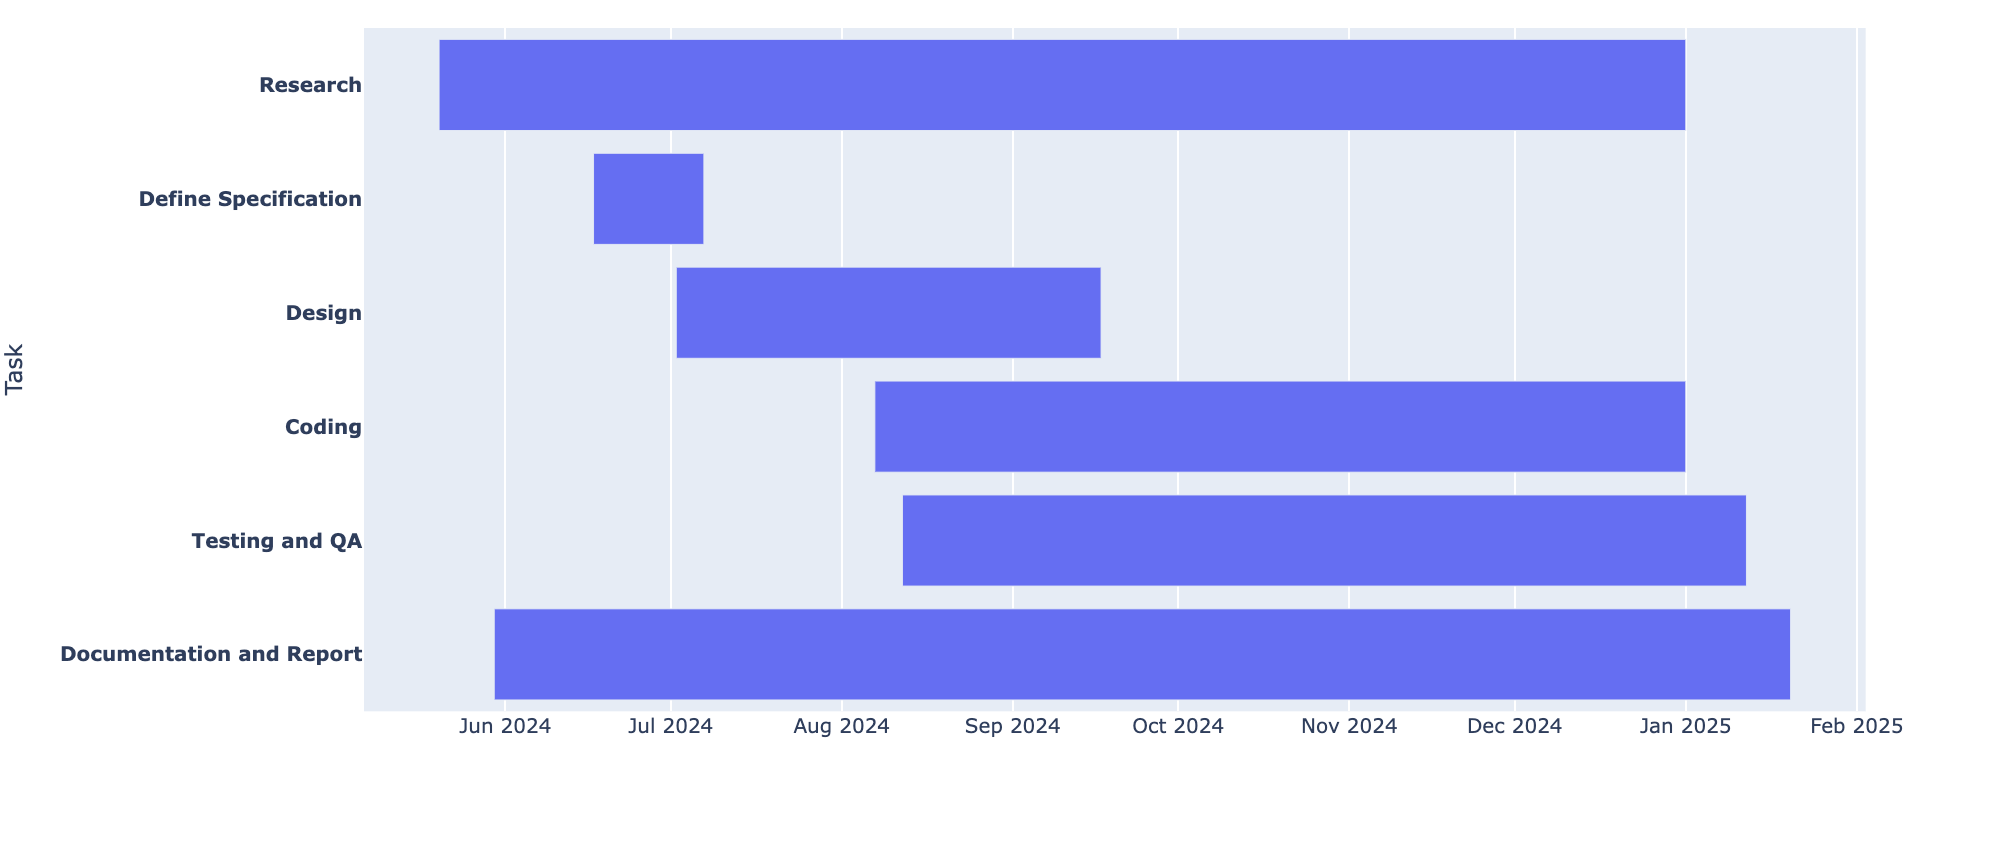
\includegraphics[scale=0.4]{images/GanttChart.png}
    \caption{Gantt Chart}\label{fig:my_label}
\end{figure}
\newpage
\section{System Requirements}

\subsection{Development Requirements}
\begin{table}[h]
    \centering
    \caption{Development Requirements}
    \begin{tabular}{|l|l|}
        \hline
        \textbf{Software Requirements}                 & \textbf{Hardware
        Requirements}                                                          \\ \hline
        Programming Language: Python, Dart, Javascript & RAM: \(>\)= 8 GB
        Megapixels                                                             \\ \hline
        Design Tools: Figma, Canva, Draw.io            & CPU: i5 10th 
        \\ \hline
        Libraries: Librosa, PyAudio, Pytorch           & GPU: P100
        (Recommended)                                                          \\ \hline
        Framework: Flutter, Django RestFramework       & Storage: \(>\)= 50 GB
        \\ \hline
        IDEs: VSCode, Android Studio                  &
        \\ \hline
    \end{tabular}
\end{table}

\subsection{Deployment Requirements}
\begin{table}[ht]
    \centering
    \caption{Deployment Requirements}
    \begin{tabular}{|l|l|}
        \hline
        \textbf{Software Requirements} & \textbf{Hardware Requirements}
        \\ \hline
        Android: \(>\)= 10             & RAM: \(>\) 4 GB
        \\ \hline
        Read/Write FileSystem          & Storage: \(>\)= 20 GB
        \\ \hline
        Internet Accessibility         & Recording Quality \(>\)= 256 Kbps, 48
        KHz 
        \\ \hline
        Database: Sqlfite              &                                                               \\ \hline
    \end{tabular}
\end{table}

\chapter{Literature Review}

This literature review explores the progression of methodologies and
technologies in the field,
with a particular focus on the use of Convolutional Neural Networks (CNN) and
Long Short-Term Memory (LSTM)
networks for audio-based bird species identification. The review also examines
the challenges associated
with dataset quality and diversity, and the innovative strategies employed to
address these issues,
providing a comprehensive overview of the current state of research and future
directions in avian bioacoustics.

\section{Related Works}
BirdNET is a cutting-edge research platform developed through collaboration
between the K. Lisa Yang Center for Conservation Bioacoustics at the Cornell
Lab of Ornithology and the Chair of Media Informatics at Chemnitz University of
Technology. Its primary aim is to detect and classify bird sounds using machine
learning technologies, serving both experts and citizen scientists in their
efforts to monitor and protect bird populations.\\\\ BirdNET can identify
around 3,000 of the world's most common bird species, with plans to expand this
number. Features such as a live submissions map and a Twitter bot are included
to engage the community and share real-time data. The project is supported by
donations and collaborations, offering opportunities for researchers and
developers to contribute to its growth. BirdNET serves as an invaluable tool
for bird enthusiasts, conservationists, and biologists alike, providing
innovative solutions for large-scale acoustic monitoring and contributing to
the conservation and understanding of avian biodiversity.\\\\ The BirdCLEF 2023
competition on Kaggle is a significant data science challenge that falls under
the broader LifeCLEF initiative, aimed at pushing the boundaries of species
identification and biodiversity monitoring through technological innovation.
This particular competition focuses on the development of machine learning
models that can identify bird species based on audio recordings. It presents a
complex and realistic challenge due to the diversity of the audio recordings,
which are collected from various environments and feature a wide range of bird
species.
\section{Related Research}

The study\cite{gautam2023audio} "Audio Classifier for Automatic Identification of Endangered Bird Species
of Nepal" focuses on using deep learning techniques to identify endangered bird species from 
audio recordings. The dataset, collected from xeno-canto.org, comprises 2215 audio recordings 
of 41 bird species, 38 of which are endangered. This dataset was expanded to 6733 recordings 
through 10-second audio splitting and Gaussian noise augmentation, with 5407 recordings used for 
training, 639 for validation, and 687 for testing. The methodology involved handling imbalanced 
class distribution through data augmentation, employing Mel spectrograms and Mel-Frequency Cepstral 
Coefficients (MFCCs) for feature extraction, and developing a custom Convolutional Neural Network (CNN) 
model and an EfficientNet model. The hyperparameters of these models were optimized using a genetic
 algorithm. The Mel spectrograms were created using Short-Time Fourier Transform, converting amplitudes 
 to decibel scale, and applying Mel filter banks to the spectrograms. Similarly, MFCCs were derived by 
 framing the audio signals, applying Discrete Fourier Transform, logarithmic scaling, Mel scaling, and 
 Discrete Cosine Transform. The EfficientNet architecture utilized compound scaling for network depth, 
 width, and resolution. The findings indicated that the proposed approach achieved satisfactory results 
 in classifying the bird species. Model I, using Mel Spectrogram and EfficientNet, achieved an F1-score of 
 79\%, while Model II, using Mel Spectrogram and Custom CNN, achieved 64\%, and Model III, using MFCC and 
 EfficientNet, achieved 72\%. However, limitations include the relatively small dataset size and the need 
 for further enhancement in model robustness and accuracy. 
%Future enhancements could involve
% expanding the dataset, exploring additional feature extraction techniques, and
% incorporating more advanced deep learning models to improve classification
% performance.\cite{gautam2023audio}\\

Sevilla et al.\cite{sevilla2017audio} introduced an innovative approach to bird sound classification with their study
`Audio Bird Classification with Inception-v4 extended with Time and
Time-Frequency Attention Mechanisms'. The datasets employed include
various bird sounds, prominently from the BirdClef2017 challenge, consisting of
1500 bird species recordings. The methodology revolves around treating bird
sound classification as an image classification problem through transfer
learning. The Inception-v4 model, initially pre-trained on ImageNet, was
adapted to process time-frequency representations of bird sounds by converting
these sounds into RGB images using three log-spectrograms generated via fast
Fourier transform at different scales (128, 512, 2048 bins).The findings
demonstrate that the model,
termed `Soundception', integrates time and time-frequency attention mechanisms
effectively, significantly improving classification accuracy. The results
highlight Soundception's outstanding performance, achieving a mean average
precision (MAP) of 0.714 in classifying 1500 bird species, 0.616 MAP for
background species, and 0.288 MAP for soundscapes with time-codes, making it
the top model in the BirdClef2017 challenge across multiple tasks. However,
limitations include the incomplete convergence of the model due to
computational constraints and the extensive GPU resources required for
training. The paper concludes with a discussion on future
improvements, such as exploring different scalable optimizations and
incorporating stacked GRU layers for better audio-to-image representation
learning, underscoring the potential of transfer learning from advanced image
classification models to acoustic domains.\\

The study, conducted by Chandu B et al.\cite{chandu2020automated}, 
outlines a robust methodology for identifying bird
species from audio recordings, leveraging a combination of meticulously curated
datasets and  machine learning techniques. The dataset was manually compiledThe working mechanism for bird identification from audio utilizes the dataset compiled from Xeno Canto, housing a diverse collection of avian vocalizations. 
Our methodology revolves around the utilization of EfficientNet, a state-of-the-art convolutional neural network architecture known for 
its balance between accuracy and efficiency.

The primary objective of this study is to achieve high levels of accuracy in identifying a broad spectrum of 41 distinct bird species. 
Here lies the detailed explanation of the methodology, from the working mechanism to model training.
from both local recordings and
online resources such as xeno-canto.org, which apart from bird songs also
contains ambient noise and
human voices to simulate real-world conditions. Pre-processing techniques
including pre-emphasis, framing, silence removal, and reconstruction were
applied to the audio clips to enhance the relevant frequency components and
eliminate unnecessary noise, ensuring the purity of the dataset. Spectrograms
of these processed clips were generated and used as input for training a
convolutional neural network (CNN), specifically AlexNet, chosen for its high
accuracy in image classification tasks. Through transfer learning, AlexNet was
adapted to recognize bird species from the spectrograms, achieving a
classification accuracy of 97\% in controlled environments. However,
recognizing the variability of real-world conditions, the researchers retrained
the model with datasets containing ambient noise, achieving a real-time
classification accuracy of 91\%. Despite these promising results, the study
acknowledges limitations such as the relatively small size of the dataset and
the need for further tuning of performance parameters to improve
robustness.\\

In\cite{nanni2021ensemble} `An Ensemble of Convolutional Neural Networks for Audio
Classification' delves into a comprehensive study on CNN classification using
different architectures, data augmentation techniques, and audio signal
representations, aimed at enhancing audio classification tasks across various
datasets. The study employs three datasets: BIRDZ, CAT, and ESC-50, each
offering unique challenges in audio classification. The methodology involves
training five convolutional neural networks (CNNs) with four audio
representations combined with six different data augmentation methods,
resulting in thirty-five subtypes of ensembles. The audio representations
include techniques such as the Discrete Gabor Transform (DGT), Waveform
Similarity OverLap Add (WSOLA), and Phase Vocoder. The data augmentation
methods encompass procedures like short spectrogram augmentation, random time
shift, and frequency masking. The CNN architectures are pre-trained models
fine-tuned with these augmented datasets to boost classification accuracy. The
findings reveal that the ensemble method outperforms standalone networks,
achieving 97\% accuracy on the BIRDZ dataset, 90.51\% on the CAT dataset, andThe working mechanism for bird identification from audio utilizes the dataset compiled from Xeno Canto, housing a diverse collection of avian vocalizations. 
Our methodology revolves around the utilization of EfficientNet, a state-of-the-art convolutional neural network architecture known for 
its balance between accuracy and efficiency.

The primary objective of this study is to achieve high levels of accuracy in identifying a broad spectrum of 41 distinct bird species. 
Here lies the detailed explanation of the methodology, from the working mechanism to model training.
88.65\% on the ESC-50 dataset. The study also highlights that the
best-performing CNNs are VGG16 and VGG19, with DGT as the most effective signal
representation. However, the study acknowledges limitations, such as the
computational cost of training ensembles and the variability in performance
across different augmentation techniques.\\

In\cite{wang2022efficient} `Analysis of bird call datasets sourced
from Xeno-Canto', comprising 72,172 samples from 264 bird species in 16-bit wav
format with a 16 kHz sampling rate. The methodology involved preprocessing the
audio data to filter out low-frequency noise and normalize signal amplitude,
followed by generating Mel-spectrograms and Mel-Frequency Cepstral Coefficients
(MFCCs) as inputs for deep learning models. The Mel-spectrograms were produced
using discrete Fourier transform (DFT), and the MFCCs were derived by applying
discrete cosine transform (DCT) to the Mel-spectrogram. The study employed
various metrics to evaluate the performance of these methods, including ROC
analysis to visualize model effectiveness. Findings indicated that the proposed
models showed significant promise in identifying bird species from their calls,
with improvements in classification accuracy compared to previous approaches.
However, limitations were noted, including potential biases in the dataset due
to uneven sample distribution across species and the challenge of background
noise affecting signal quality. Future work suggested enhancing noise reduction
techniques and exploring more sophisticated neural network architectures to
further improve model robustness and accuracy.\\

The study\cite{pahuja2021sound} by Pahuja et al. conducted an in-depth analysis of bird species recognition through
acoustic monitoring, utilizing a robust dataset of bird sound samples,
meticulously annotated and validated for accuracy. The dataset, referred to as
SD, comprises multispecies bird sound recordings, each labeled with species
name and sample ID, along with corresponding metadata, providing a
comprehensive foundation for model training and evaluation. Methodologically,
the research employed a spectrogram-based feature extraction approach,
leveraging Short-Time Fourier Transform (STFT) to capture the intricate
temporal and spectral characteristics of bird sounds. This was followed by the
application of a Multilayer Perceptron (MLP) classifier to distinguish between
different bird species. The findings reveal that the proposed model achieved
high recognition accuracy, with some species being identified with perfect
precision, recall, and accuracy (100\%), though the performance varied across
species, with a few showing lower recognition rates (86.9\%) and
precision/recall values ranging between 50\-75\%. The results demonstrated an
overall classification accuracy of 96\%, with cross-validation accuracy
standing at 81.4\%, highlighting the model's robustness yet indicating room for
improvement in generalizability across diverse datasets. Despite the promising
results, the study acknowledges several limitations, including the variability
in recognition accuracy among different species and the potential influence of
environmental noise on model performance. Future work is suggested to explore
feature and model fusion techniques, integrate the model with cloud-based
systems for real-time recognition, and expand the dataset to include a broader
range of bird species to enhance the model's applicability and accuracy in
practical scenarios.\\ 

The dataset used in this study\cite{carvalho2023automatic} comprises recordings labeled by species from California 
and Nevada, USA. It includes 91 species, with 30 audio samples per species, amounting 
to a total of 2,730 MP3 files. The methodology adopted involves three main steps: 
pre-processing, feature extraction, and deep learning modeling.
For feature extraction, MFCCs were obtained using the Python library python\_speech\_features, 
with parameters such as sample rate, 13 cepstrum coefficients, 26 filterbank filters, and an 
FFT size of 512. Mel spectrograms were extracted using the Librosa library, employing parameters 
such as a sample rate, an FFT window size of 2048, a hop length of 512, and 128 Mel bands.
In the deep learning modeling, CNNs and LSTMs were compared for their effectiveness in 
classifying bird sounds. CNNs demonstrated superior training accuracy with Mel spectrogram 
features, achieving 99.05\% and 98.76\% accuracy for 3-second and 1.5-second spectroThe working mechanism for bird identification from audio utilizes the dataset compiled from Xeno Canto, housing a diverse collection of avian vocalizations. 
Our methodology revolves around the utilization of EfficientNet, a state-of-the-art convolutional neural network architecture known for 
its balance between accuracy and efficiency.

The primary objective of this study is to achieve high levels of accuracy in identifying a broad spectrum of 41 distinct bird species. 
Here lies the detailed explanation of the methodology, from the working mechanism to model training.grams, 
respectively. In contrast, LSTMs achieved lower training accuracies of 75.85\% and 73.29\% 
under similar conditions.These results highlight the superior ability of CNNs to leverage 
the spatial and frequency-related patterns in Mel spectrograms for accurate bird species 
classification.\\ 

In the study\cite{lasseck2018acoustic}, 'Acoustic Bird Detection with Deep Convolution Neural Network', DCNNs pretrained 
on ImageNet, have been widely used for bioacoustic classification, with preprocessing and 
augmentation playing crucial roles in model performance. The preprocessing pipeline typically 
involves applying a shallow high-pass filter (Q = 0.707) with a 2 kHz cutoff, resampling to 22,050 Hz, 
and extracting around 4-second audio chunks, which are transformed into mel spectrograms with 310 mel bands 
(160-10,300 Hz). Further processing includes removing extreme frequencies, normalizing power 
spectrograms to decibel units, resizing to 224*224, and converting grayscale spectrograms to RGB 
for compatibility with ResNet. To improve generalization, data augmentation techniques such as 
jittering chunk duration, extracting chunks from random positions, adding noise from unrelated audio 
files, and applying random amplitude scaling are employed. Additional augmentations in the frequency 
domain include frequency shifting/stretching, piecewise time/frequency resizing, and color jittering 
(brightness, contrast, saturation, hue). Among these, the most effective methods are noise addition 
from random files, piecewise time and frequency stretching, and time interval dropout, which enhance 
robustness by simulating real-world variations in bird vocalizations.\\

\chapter{Methodology}
% \section*{}
This chapter describes the overall system including the bird sound detection and bird species classification.

\section{System Overview}
\begin{figure}[h!]
    \centering
    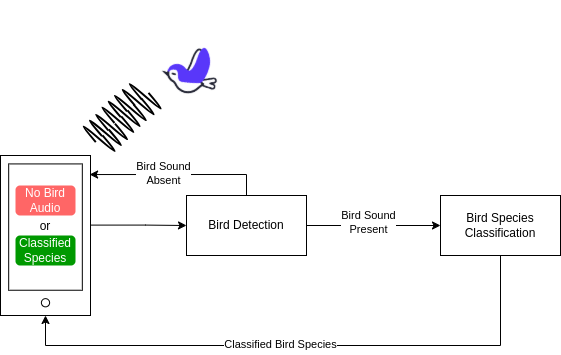
\includegraphics[scale=0.65]{images/System Overview.png}
    \caption{System Overview}%\label{fig:fig1}
\end{figure}

Our project leverages a mobile application to capture audio recordings, which are then processed to identify bird species. The mobile app records the sound and visualizes it with waveforms during the recording process. Once the audio is captured, it is sent to our backend system for further analysis.

The backend system, built using Django and Django Rest Framework, first passes the audio through a bird sound detection model. This model determines whether the recorded audio contains bird sounds. If bird sounds are detected, the audio is then forwarded to the bird species classifier model. The classifier identifies the specific bird species present in the recording.

Upon successful classification, the system maps the identified bird species to the location where the audio was recorded, utilizing the device's GPS data. This information is stored in a MySQL database, which handles all data management tasks. If the bird sound detection model does not detect any bird sounds, the recorded audio is labeled accordingly, indicating the absence of bird sounds.

This approach ensures that only relevant audio recordings are processed for species classification, enhancing the accuracy and efficiency of the system. The integration of Django, Django Rest Framework, and MySQL provides a robust and scalable backend infrastructure to support the application's functionality.
\\

\section{Working Mechanism for Detection using Audio}
The working mechanism for bird identification from audio utilizes the dataset compiled from Xeno Canto, housing a diverse collection of avian vocalizations. 
Our methodology revolves around the utilization of EfficientNet, a state-of-the-art convolutional neural network architecture known for 
its balance between accuracy and efficiency.

The primary objective of this study is to achieve high levels of accuracy in identifying a broad spectrum of 41 distinct bird species. 
Here lies the detailed explanation of the methodology, from the working mechanism to model training.
\begin{figure}[h!]
    \centering
    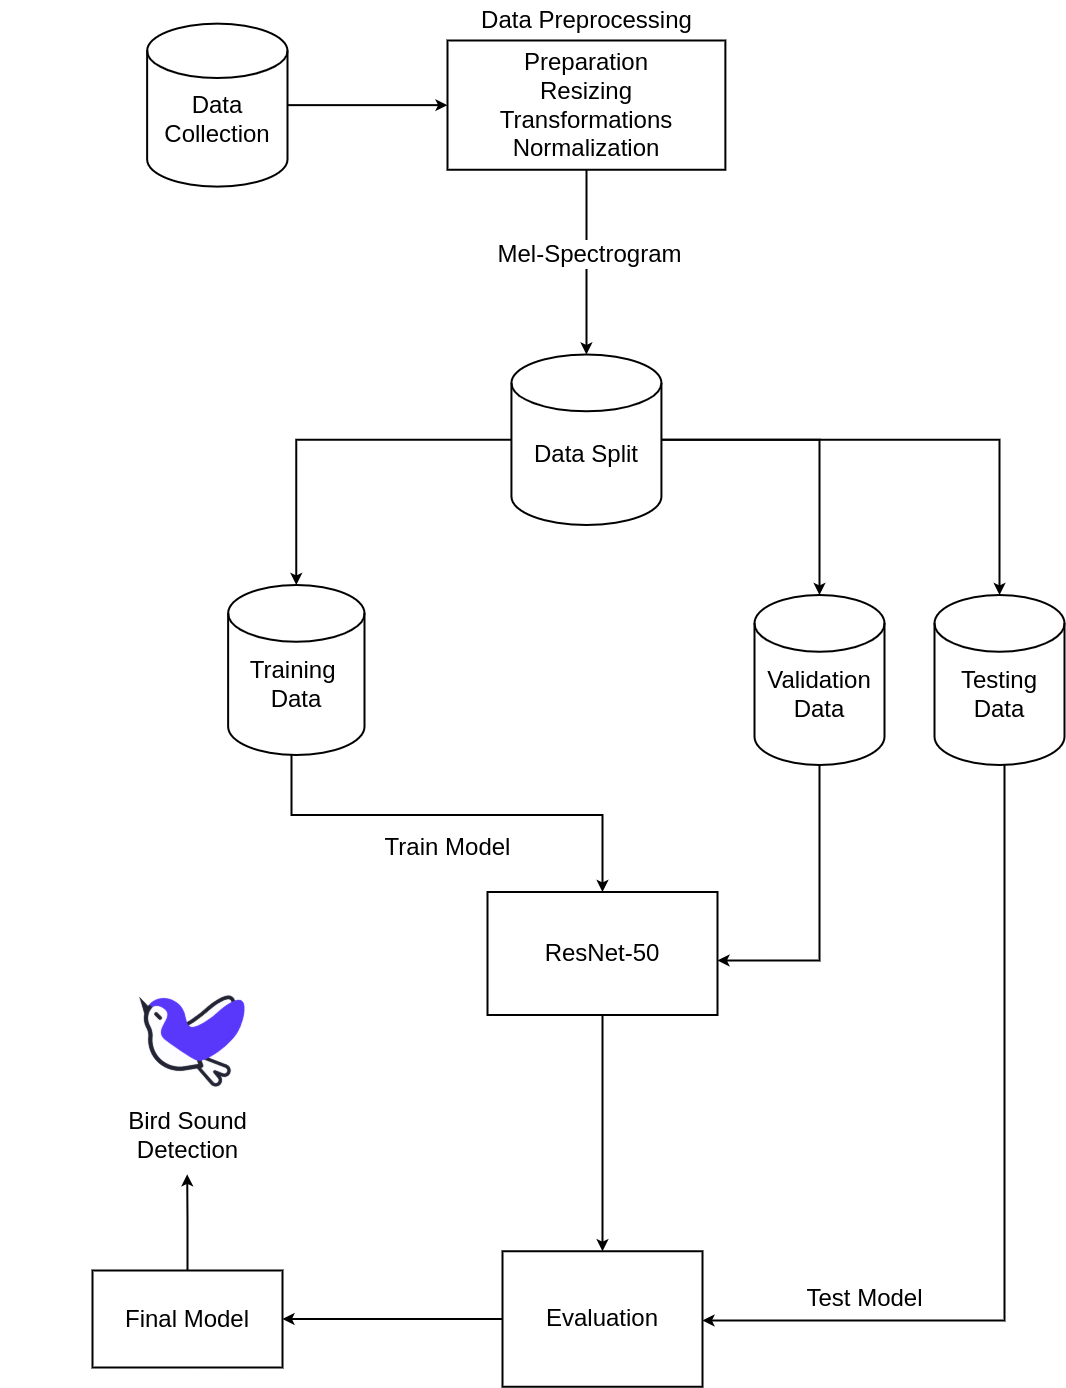
\includegraphics[scale=0.33]{images/DetectionMethodology.png}
    \caption{Block diagram for the working mechanism for Bird Detection}%\label{fig:fig1}
\end{figure}


\section{Working Mechanism for Identification using Audio}
The working mechanism for bird identification from audio utilizes the dataset compiled from Xeno Canto, housing a diverse collection of avian vocalizations. 
Our methodology revolves around the utilization of EfficientNet, a state-of-the-art convolutional neural network architecture known for 
its balance between accuracy and efficiency.

The primary objective of this study is to achieve high levels of accuracy in identifying a broad spectrum of 41 distinct bird species. 
Here lies the detailed explanation of the methodology, from the working mechanism to model training.
% https://www.geeksforgeeks.org/vgg-16-cnn-model/
\begin{figure}[h!]
    \centering
    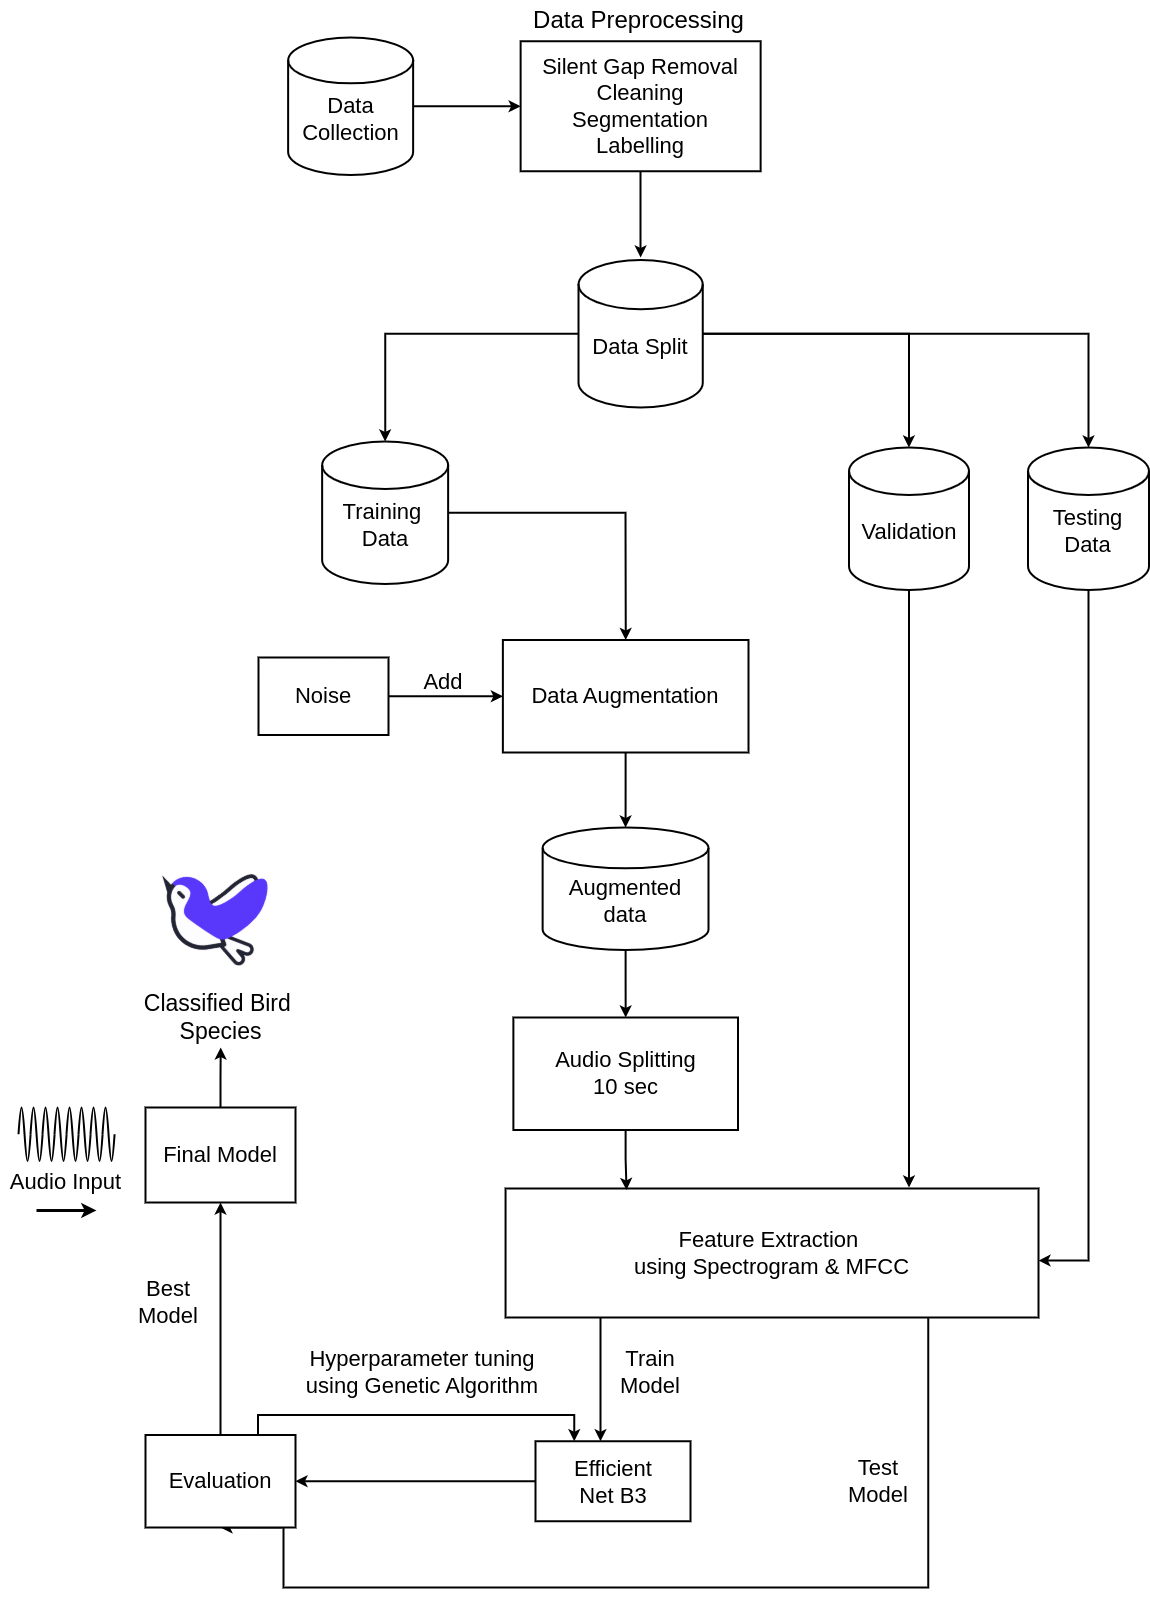
\includegraphics[scale=0.33]{images/IdentificationMethodology.png}
    \caption{Block diagram for the working mechanism for Bird Species Identification}%\label{fig:fig1}
\end{figure}
\newpage

\subsection{Dataset}
For this project, we scraped audio data from Xeno-canto (\textit{xeno-canto.org}), a global repository of bird vocalizations contributed 
by ornithologists and birding enthusiasts. Since the dataset was highly imbalanced, we applied a series of preprocessing and augmentation 
techniques to ensure a more uniform distribution across bird species.

\begin{figure}[h!]
    \centering
    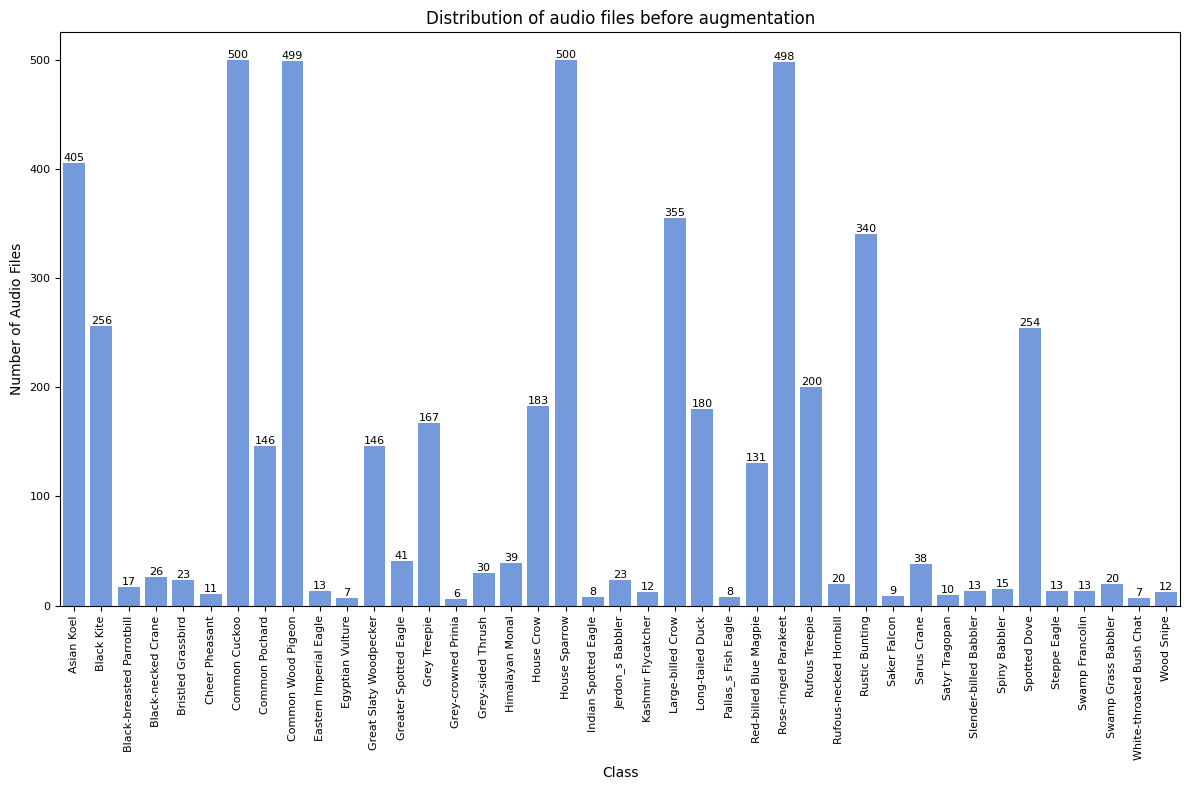
\includegraphics[width=0.8\textwidth]{images/before_augmentation.png}
    \caption{Data before performing augmentation}
    \label{fig:visualization}
\end{figure}
\newpage


\subsection{Data Augmentation}
Initial analysis of the collected data revealed significant class imbalance, with some species having over 400 recordings while others had fewer than 50. Additionally, the audio recordings varied in length. To address these issues:  
\begin{itemize}
    \item \textbf{Audio Clipping:}  
    \begin{itemize}
        \item Recordings were clipped into segments of 10 seconds each.  
        \item Clips shorter than 5 seconds were discarded to avoid blank audio segments and insufficient data.  
        \item Clips between 5 and 10 seconds were padded with silence at the end to standardize their length to 10 seconds.  
    \end{itemize}

    \item \textbf{Augmentation Techniques:}  
    To balance the dataset, augmentation techniques such as time stretching, phase shifting, and noise addition were applied. The parameters were varied to ensure diversity in the augmented data.  
    \begin{itemize}
        \item Each bird class was augmented to contain exactly 500 audio clips.
    \end{itemize}
\end{itemize}

\begin{figure}[h!]
    \centering
    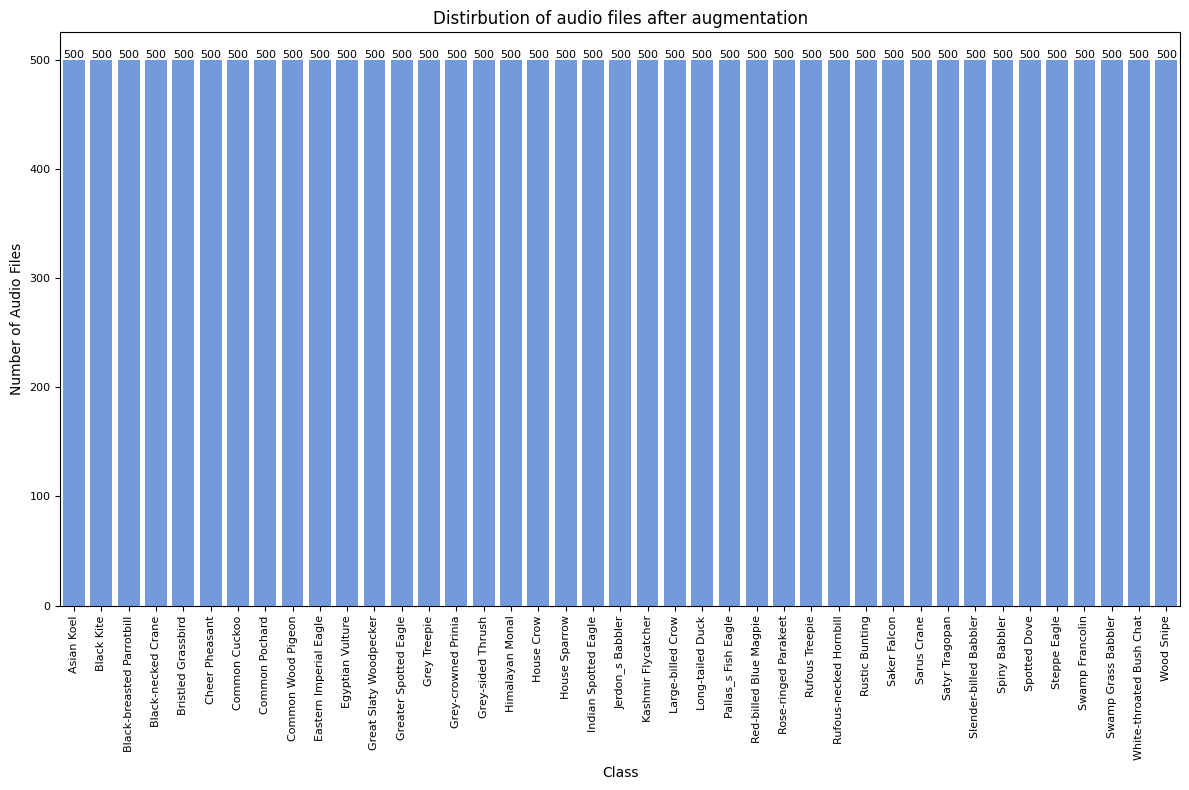
\includegraphics[width=0.8\textwidth]{images/after_augmentation.png}
    \caption{Data after performing augmentation}
    \label{fig:visualization}
\end{figure}



\newpage


% \subsection{Dataset}
% For this project, we scraped audio data from Xeno-canto (\textit{xeno-canto.org}), a global repository of bird vocalizations contributed 
% by ornithologists and birding enthusiasts. Since the dataset was highly imbalanced, we applied a series of preprocessing and augmentation 
% techniques to ensure a more uniform distribution across bird species.

% First, we split all audio files into 10-second segments. For recordings that were between 5 and 10 seconds, we padded them to make all audio 
% files exactly 10 seconds long. To further augment the dataset and improve model generalization, we applied time stretching, phase shifting, 
% and Gaussian noise addition to the audio samples.

% At the end of this process, we obtained a balanced dataset consisting of 500 audio files per class across 41 bird species, ensuring a more 
% robust and effective training set for our model.
% \newpage

% \subsection{Dataset Overview for Audio}
% \begin{figure}[h!]
%     \centering
%     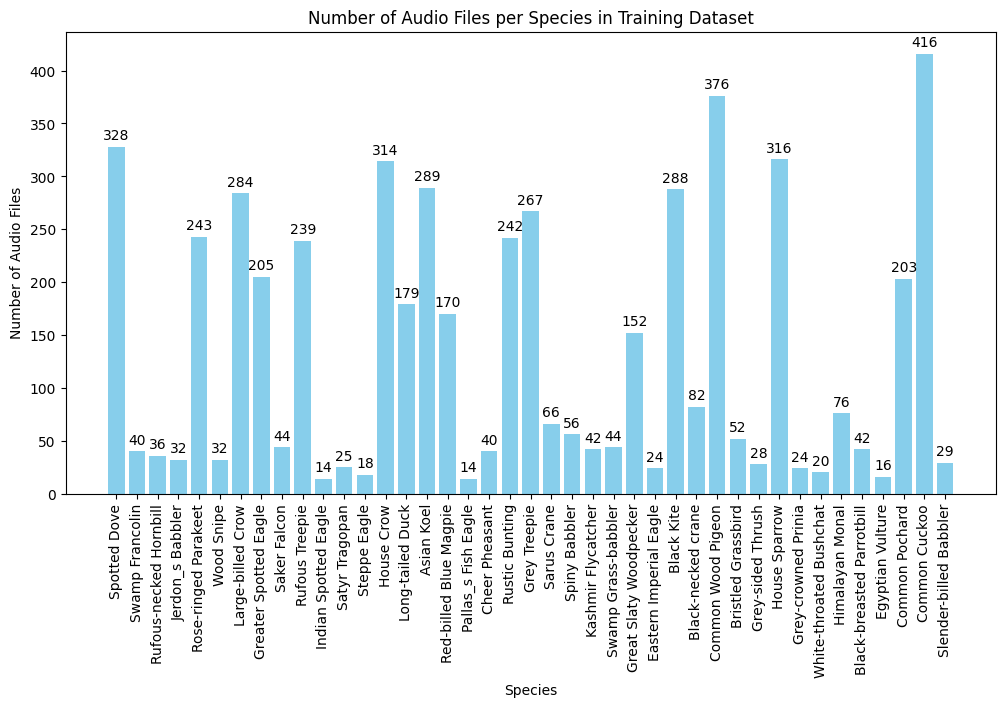
\includegraphics[scale=0.4]{images/TrainingDataset.png}
%     \caption{Training Dataset for audio}
% \end{figure}

% \begin{figure}[h!]
%     \centering
%     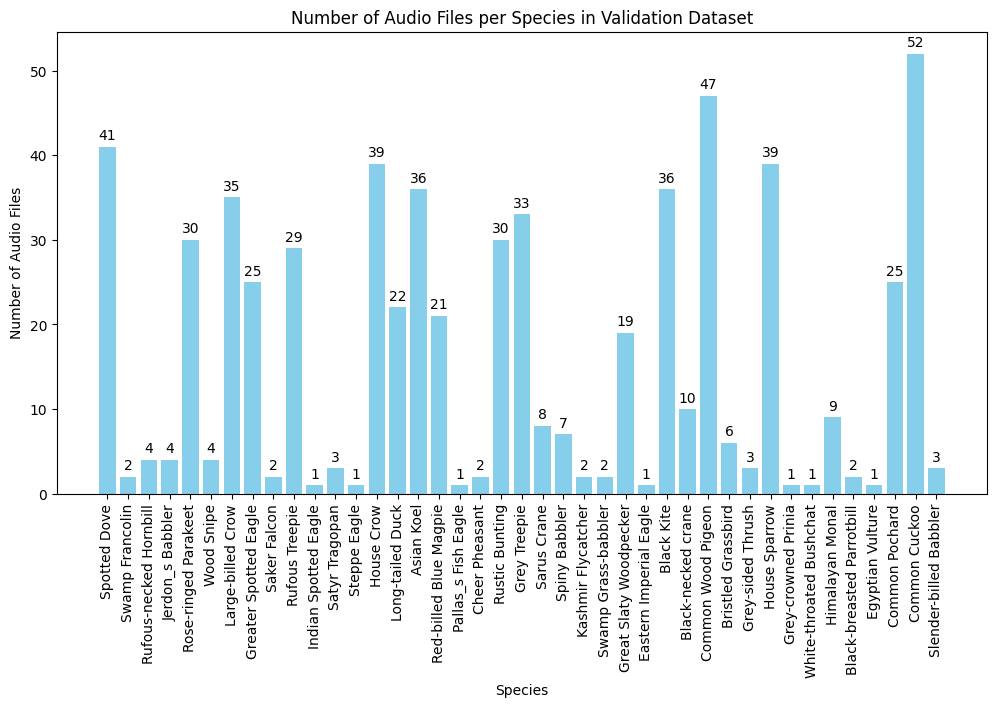
\includegraphics[scale=0.4]{images/ValidationDataset.png}
%     \caption{Validation Dataset for audio}
% \end{figure}
% \newpage
% \begin{figure}[h!]
%     \centering
%     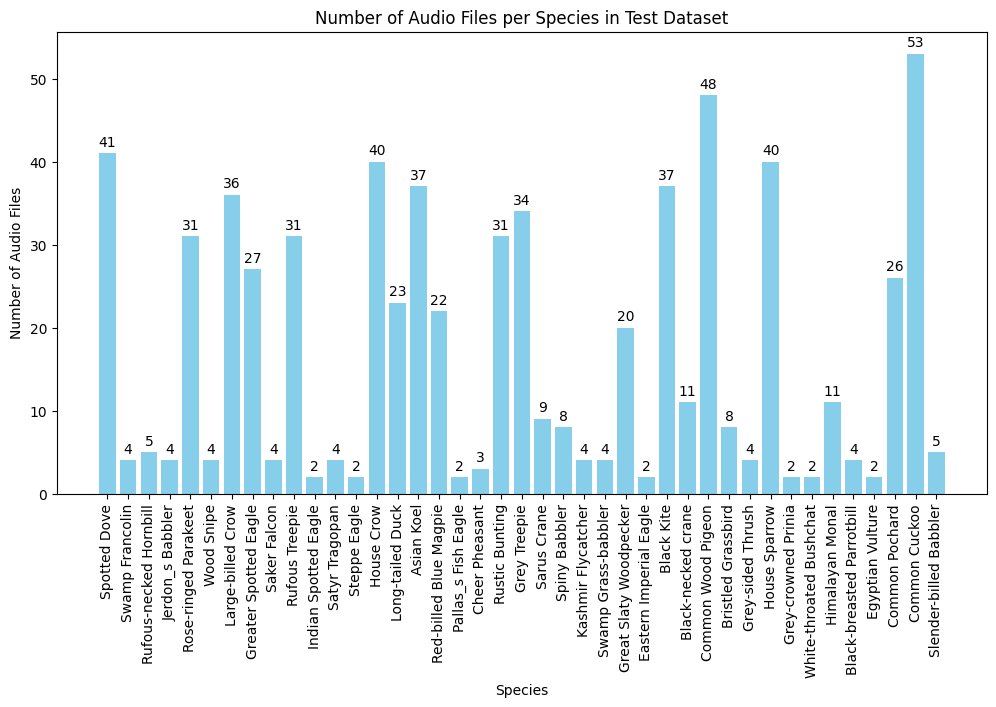
\includegraphics[scale=0.4]{images/TestDataset.png}
%     \caption{Testing Dataset for audio}
% \end{figure}
% \hspace{3.5cm}
% \begin{figure}[h!]
%     \centering
%     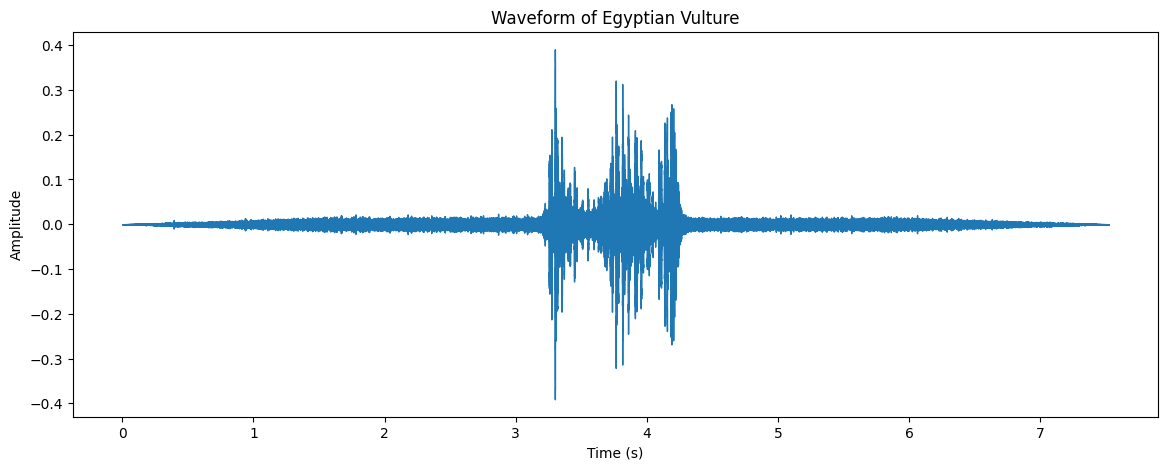
\includegraphics[scale=0.3]{images/SampleData.png}
%     \caption{Sample of the Data}
%     \label{fig:SampleData}
% \end{figure}
% \newpage

% \subsection{Dataset Overview for Audio}
% \begin{figure}[h!]
%     \centering
%     \includegraphics[scale=0.4]{images/PreAugmentation.png}
%     \caption{Distribution of data before augmentation}
% \end{figure}

% \begin{figure}[h!]
%     \centering
%     \includegraphics[scale=0.4]{images/PostAugmentation.png}
%     \caption{Distribution of data after augmentation}
% \end{figure}
% \newpage

% \subsection{Data Preprocessing}

% The collected audio data undergoes thorough preprocessing to ensure its
% suitability for model training. This process includes:
% \begin{itemize}
%     \item \textbf{Silence Gap Removal:} After observing some of the data
%           samples, it was found that the audio has some silence gaps
%           in either of the ends as seen in \ref{fig:SampleData}. These could be
%           removed employing the silence removal algorithm. The processing
%           starts from both ends and moves toward the center. In that processing,
%           the local mean of the window segment of the audio wave is
%           calculated and compared with the audio's global mean. If the local mean
%           is smaller than the global mean, the window segment is c
%           onsidered to contain insignificant data, thus the segment is clipped
%           from the original audio\cite{9850832}. Algorithm \ref{alg:Silence_Removal}
%           clarifies this.
%     \item \textbf{Segmentation:} Dividing the continuous audio recordings into
%           smaller, more manageable segments, ensuring consistency in input length.
%     \item \textbf{Cleaning:} Removing any background noise and irrelevant
%           sounds that could interfere with the training process.
%     \item \textbf{Labeling:} Assigning the correct bird species labels to each
%           audio segment, which is crucial for supervised learning.
% \end{itemize}

% \subsection{Data Splitting}

% After preprocessing, the data is split into three sets:
% \begin{itemize}
%     \item \textbf{Training Data:} Used to train the machine learning models.
%     \item \textbf{Testing Data:} Used to evaluate the model's performance
%           during training.
%     \item \textbf{Validation Data:} Used to validate the final model's
%           performance and prevent overfitting.
% \end{itemize}

% This structured approach ensures that the model can learn effectively from the
% training data while being evaluated on unseen data to measure its
% generalization capabilities.

% \subsection{Data Augmentation}

% To further enhance the robustness of the model, data augmentation techniques
% are applied to the training data. This includes adding various types of noise
% to the audio segments to create more diverse training samples and prevent the
% model from overfitting to specific patterns in the data.
% \begin{eqnarray}
%     \text{Augmented Data} = \text{Original Data} + \text{Noise}
% \end{eqnarray}

% By introducing these variations, the model becomes more resilient to different
% audio conditions and better at generalizing to new recordings.

% \subsection{Audio Splitting}

% The augmented audio data is then split into smaller 10-second clips. This
% standardization ensures that the input size remains consistent, which is
% essential for the feature extraction and modeling stages.


\subsection{Data Preprocessing}
The audio recordings were transformed into Mel Spectrograms for further analysis.  

\begin{itemize}
    \item \textbf{Conversion Details:}  
    \begin{itemize}
        \item Audio files were converted using a sample rate of 32,000 Hz.  
        \item The spectrograms were generated with a Hanning window and 48 Mel bands.  
    \end{itemize}

    \item \textbf{Dataset Expansion:}  
    \begin{itemize}
        \item Each of the 500 audio files per bird class was converted into corresponding Mel Spectrogram images.  
        \item The resulting dataset was divided into training, validation, and testing sets for model development.
    \end{itemize}
\end{itemize}

\subsection{Model Training}  
The classification model was built using \textbf{EfficientNetB3} as the base architecture.  

\begin{itemize}
    \item \textbf{Input Preprocessing:}  
    \begin{itemize}
        \item Mel Spectrogram images were resized to \(128 \times 128 \times 3\) and normalized using the preprocess\_input function of EfficientNet.  
    \end{itemize}

    \item \textbf{Regularization:}  
    \begin{itemize}
        \item Dropout layers and kernel regularizers were employed to mitigate overfitting.  
    \end{itemize}

    \item \textbf{Callback Functions:}  
    \begin{itemize}
        \item Early stopping, learning rate reduction on plateau, and checkpoint saving mechanisms were implemented to enhance training efficiency and performance.  
    \end{itemize}

    \item \textbf{Performance:}  
    \begin{itemize}
        \item On the test set, the model achieved an accuracy of \textbf{89.36\%} with a cross-entropy loss of \textbf{0.42}.  
    \end{itemize}
\end{itemize}

\subsection{Genetic Algorithm for Hyperparameter Tuning}
To optimize the performance of our model, we used genetic algorithm for hyperparameter tuning. 
This approach helped us systematically explore and identify the most effective hyperparameter settings for our model, 
including learning rates, batch sizes, and network architecture parameters. 
The genetic algorithm enabled a more efficient and comprehensive search for optimal configurations.

\subsection{Feature Extraction}
Feature extraction is a critical step where the audio clips are transformed
into a format that can be fed into machine learning models. We use two primary
techniques for feature extraction: Spectrograms and Mel-Frequency Cepstral
Coefficients (MFCC).

\subsubsection{Spectrogram}
A spectrogram is a visual representation of the spectrum of frequencies in a
sound signal as they vary with time. It is generated by applying the Short-Time
Fourier Transform (STFT) to the audio signal. This transformation provides
insight into how the frequency content of the signal changes over time.
\begin{eqnarray}
    X(n) = \sum_{m=0}^{N-1} x(m) \cdot w(n-m)
\end{eqnarray}
% \[
% X(n) = \sum_{m=0}^{N-1} x(m) \cdot w(n-m)
% \]

where \( x(m) \) is the audio signal and \( w(n) \) is the window function.

\subsubsection{Mel-Frequency Cepstral Coefficients (MFCC)}

MFCCs are coefficients that collectively describe the short-term power spectrum
of a sound signal. The process of obtaining MFCCs involves several steps:
\begin{figure}[h!]
    \centering
    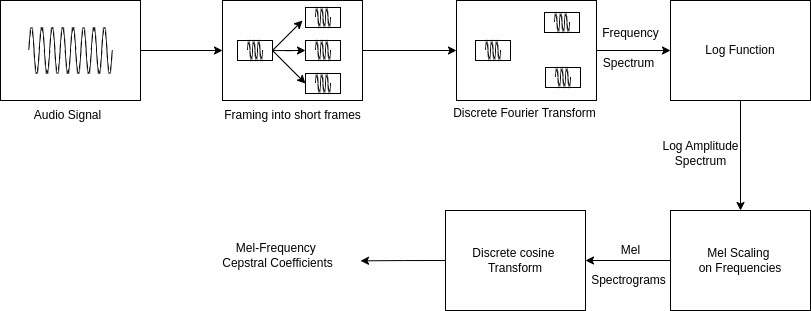
\includegraphics[scale=0.5]{images/MFCC.jpg}
    \caption{Feature Extraction Using Spectrogram and
        MFCC}%\label{fig:fig1}
\end{figure}
\begin{enumerate}
    \item \textbf{Framing:} Divide the audio signal into short frames.
    \item \textbf{Discrete Fourier Transform (DFT):} Convert each frame to the
          frequency domain.
          \begin{eqnarray}
              X(k) = \sum_{n=0}^{N-1} x(n) \cdot e^{-j \frac{2\pi}{N} kn}
          \end{eqnarray}

    \item \textbf{Log Function:} Apply a logarithm to the amplitude spectrum.
          \begin{eqnarray}
              S_{\text{log}}(k) = \log(|X(k)|)
          \end{eqnarray}

    \item \textbf{Mel-Scaling:} Map the frequencies to the Mel scale, which
          better represents how humans perceive sound.
          \begin{eqnarray}
              f_{\text{mel}} = 2595 \cdot \log_{10}(1 + \frac{f}{700})
          \end{eqnarray}

    \item \textbf{Discrete Cosine Transform (DCT):} Convert the Mel spectrum to
          the cepstral domain, yielding the MFCC features.
          \begin{eqnarray}
              C(n) = \sum_{k=0}^{K-1} S_{\text{mel}}(k) \cdot \cos \left(
              \frac{\pi n (k+0.5)}{K} \right)
          \end{eqnarray}

\end{enumerate}


\subsection{EfficientNet}
EfficientNet is a family of convolutional neural networks (CNNs) designed to achieve high accuracy with optimal computational efficiency. 
It utilizes a novel compound scaling approach, which uniformly scales depth, width, and resolution, unlike traditional models that scale 
these dimensions arbitrarily. Developed by Google, EfficientNet outperforms many previous architectures while using fewer parameters and 
lower computational costs. This makes it particularly effective for tasks like image classification and feature extraction, including applications 
in bioacoustics, where it can analyze spectrograms for bird sound identification with high precision.

\begin{figure}[h!]
    \centering
    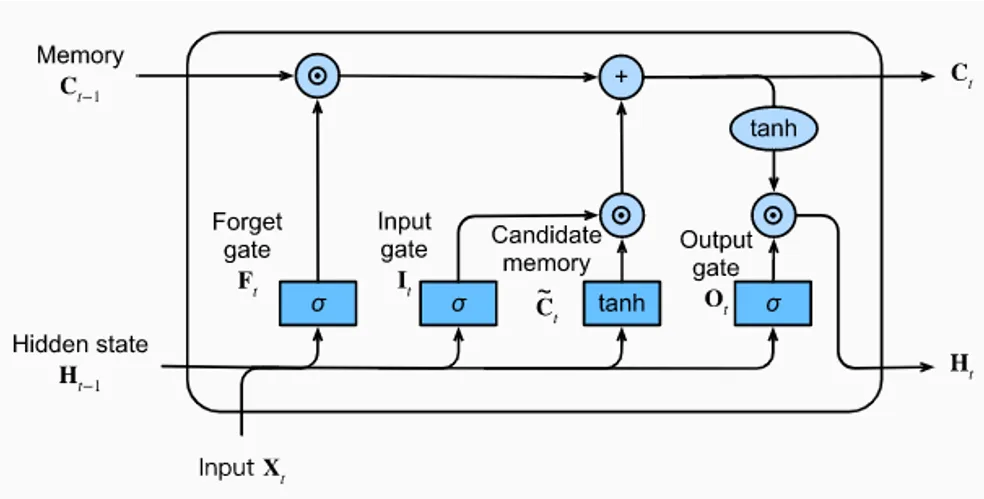
\includegraphics[scale=0.4]{images/LSTM.png}
    % citation link: https://medium.com/@ottaviocalzone/an-intuitive-explanation-of-lstm-a035eb6ab42c
    \caption{EfficientNet architecture}%\label{fig:fig1}
\end{figure}



\subsection{Convolutional Neural Networks (CNN)}

Convolutional Neural Networks (CNNs) are highly effective for extracting
spatial features from spectrograms, making them well-suited for audio
classification tasks. CNNs use convolutional layers to detect patterns and
features in the input data by applying convolutional filters across the input
spectrogram.

\begin{figure}[h!]
    \centering
    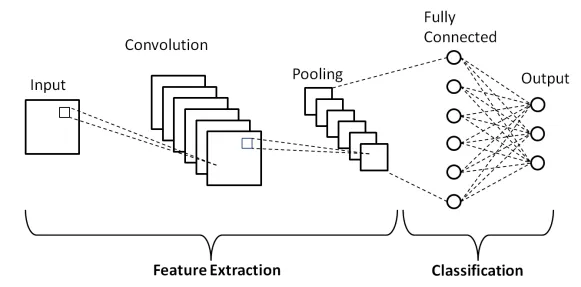
\includegraphics{images/Convolution.png}
    \caption{CNN architecture}%\label{fig:fig1}
    % citation link: https://medium.com/techiepedia/binary-image-classifier-cnn-using-tensorflow-a3f5d6746697
\end{figure}

The basic operations involved in a CNN include:
\begin{itemize}
    \item \textbf{Convolution:} This operation involves applying a set of
          learnable filters (kernels) across the input spectrogram to produce feature
          maps.
          \begin{eqnarray}
              (f * x)(t) = \sum_{\tau = -\infty}^{\infty} x(\tau) \cdot f(t -
              \tau)
          \end{eqnarray}

    \item \textbf{Activation Function:} The rectified linear unit (ReLU)
          activation function is applied to introduce non-linearity into the model.
          \begin{eqnarray}
              f(x) = \max(0, x)
          \end{eqnarray}

    \item \textbf{Pooling:} Pooling layers reduce the spatial dimensions of the
          feature maps, typically using
          max pooling to retain the most significant features.
    \item \textbf{Fully Connected Layers:} After several convolutional and
          pooling layers, the feature maps
          are flattened and passed through fully connected layers to produce the
          final classification output.
\end{itemize}

\subsection{Long Short-Term Memory Networks (LSTM)}

Long Short-Term Memory (LSTM) networks are a type of recurrent neural network
(RNN) capable of capturing temporal dependencies in sequential data. This makes
them well-suited for processing audio signals where the order of data points
matters. LSTMs are designed to overcome the limitations of traditional RNNs by
addressing the vanishing gradient problem through the use of gates that
regulate the flow of information.

\begin{figure}[h!]
    \centering
    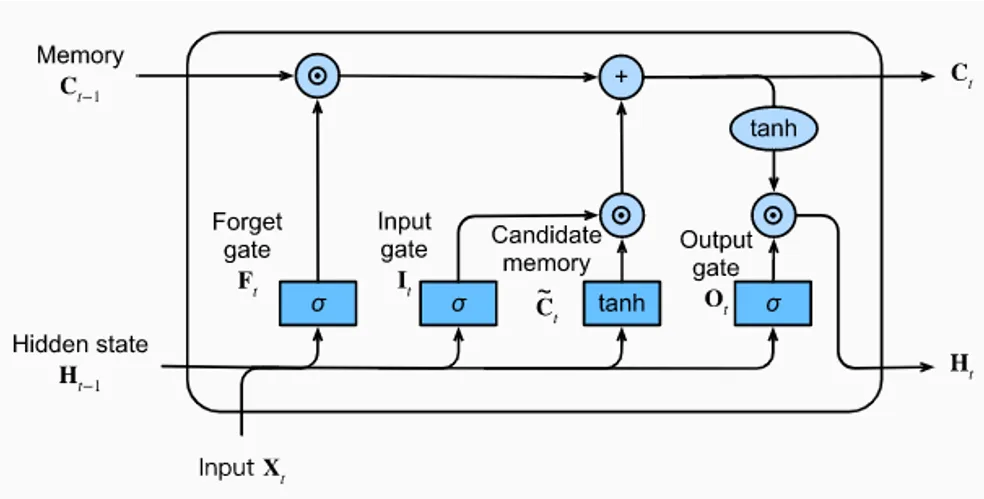
\includegraphics[scale=0.4]{images/LSTM.png}
    % citation link: https://medium.com/@ottaviocalzone/an-intuitive-explanation-of-lstm-a035eb6ab42c
    \caption{LSTM architecture}%\label{fig:fig1}
\end{figure}

The key components of an LSTM cell include:
\begin{itemize}
    \item \textbf{Forget Gate:} Determines which information from the previous
          cell state should be discarded.
          \begin{eqnarray}
              f_t = \sigma(W_f \cdot [h_{t-1}, x_t] + b_f)
          \end{eqnarray}

    \item \textbf{Input Gate:} Decides which new information should be added to
          the cell state.
          \begin{eqnarray}
              i_t = \sigma(W_i \cdot [h_{t-1}, x_t] + b_i)
          \end{eqnarray}

    \item \textbf{Candidate Cell State:} Creates new candidate values that
          could be added to the cell state.
          \begin{eqnarray}
              \tilde{C}_t = \tanh(W_C \cdot [h_{t-1}, x_t] + b_C)
          \end{eqnarray}

    \item \textbf{Cell State:} The cell state is updated based on the input
          gate and the forget gate.
          \begin{eqnarray}
              C_t = f_t \cdot C_{t-1} + i_t \cdot \tilde{C}_t
          \end{eqnarray}

    \item \textbf{Output Gate:} Determines the output of the LSTM cell.
          \begin{eqnarray}
              o_t = \sigma(W_o \cdot [h_{t-1}, x_t] + b_o)
          \end{eqnarray}
          \begin{eqnarray}
              h_t = o_t \cdot \tanh(C_t)
          \end{eqnarray}

\end{itemize}

\subsection{Combined CNN and LSTM (CNN+LSTM)}
A hybrid model that leverages the strengths of both CNN and LSTM architectures
is developed. In this combined model, the CNN processes spectrograms to extract
spatial features, which are then fed into LSTM layers to capture temporal
patterns. The integration of these two models aims to utilize both spatial and
temporal information, thereby improving the overall classification accuracy.
Fully connected layers at the end perform the final classification based on the
features extracted by both CNN and LSTM components.

\subsection{Hyperparameter Optimization using Genetic Algorithm}
Genetic algorithms (GAs) are a powerful method for optimizing hyperparameters
in machine learning models. Genetic Algorithm have proven to significantly
improve the performance metrics of the CNN model instead of using hand tuned
approach for hyperparameters. This section outlines the steps involved in using
GAs for hyperparameter optimization\cite{9058307}.
\begin{itemize}
    \item \textbf{Encoding the Hyperparameters}
          \begin{itemize}
              \item Hyperparameters are represented as a chromosome, where each
                    hyperparameter is a
                    gene in the chromosome.
              \item For example, in a neural network, a chromosome might
                    include genes for the
                    learning rate, number of layers, number of neurons per
                    layer, and activation
                    functions.
          \end{itemize}

    \item \textbf{Initial Population}
          \begin{itemize}
              \item An initial population of chromosomes is generated randomly,
                    with each
                    chromosome representing a different set of hyperparameters.
          \end{itemize}

    \item \textbf{Fitness Function}
          \begin{itemize}
              \item A fitness function is defined to evaluate the performance
                    of each set of
                    hyperparameters.
              \item This typically involves training the model with the given
                    hyperparameters and
                    measuring its performance on a validation set.
          \end{itemize}

    \item \textbf{Selection}
          \begin{itemize}
              \item Selection involves choosing the best-performing chromosomes
                    to serve as parents
                    for the next generation.
              \item Various selection methods can be employed, such as
                    tournament selection,
                    roulette wheel selection, or rank-based selection.
          \end{itemize}
          \newpage
    \item \textbf{Crossover (Recombination)}
          \begin{itemize}
              \item Crossover combines pairs of parent chromosomes to produce
                    offspring for the
                    next generation.
              \item This is done by swapping segments of parent chromosomes to
                    create new
                    chromosomes, thereby combining features of both parents.
          \end{itemize}

    \item \textbf{Mutation}
          \begin{itemize}
              \item Mutation introduces random changes to some of the genes in
                    the offspring
                    chromosomes.
              \item This helps maintain genetic diversity in the population and
                    allows the
                    algorithm to explore a broader search space.
          \end{itemize}

    \item \textbf{Replacement}
          \begin{itemize}
              \item The current population is partially or entirely replaced
                    with the new
                    generation of chromosomes, ensuring that better solutions
                    are carried forward
                    while allowing for exploration of new possibilities.
          \end{itemize}

    \item \textbf{Termination}
          \begin{itemize}
              \item The process of selection, crossover, mutation, and
                    replacement is repeated
                    until a termination criterion is met.
              \item This could be a set number of generations, convergence of
                    fitness scores, or
                    achieving a satisfactory performance level.
          \end{itemize}

    \item \textbf{Best Solution}
          \begin{itemize}
              \item The best chromosome at the end of the process represents
                    the optimal or
                    near-optimal set of hyperparameters for the model.
          \end{itemize}
\end{itemize}
\newpage

\subsection{Algorithms Used}
\subsubsection{Silent Gaps Removal}
\label{alg:Silence_Removal}
\begin{algorithm}
    \caption{Clipping of silent gaps from both ends}
    \begin{algorithmic}[1]
        \STATE $ \text{wav} \gets \text{sampled audio signal} $
        \STATE $ \Delta \gets \text{appropriate window length} $
        \STATE \text{/* In our code, $ \Delta = 500 $ for 16KHz sampling rate
            */}
        \STATE \textbf{INPUT:} $ \text{wav}, \Delta $
        \STATE \textbf{PROCESS:}
        \STATE $ \text{wavAvg} \gets \text{Average}(|\text{wav}|) $
        \STATE $ N \gets \text{Length}(\text{wav}) $

        \STATE \text{/* Removing the silent gap from the start */}
        \FOR{$ \text{idx} = 0, \Delta, 2\Delta, \ldots, N - \Delta $}
        \STATE $ \text{win} \gets \text{wav}[\text{idx} : \text{idx} + \Delta]
        $
        \STATE $ \text{winAvg} \gets \text{Average}(|\text{win}|) $
        \IF{$ \text{winAvg} > \text{wavAvg} $}
        \STATE $ \text{wav} \gets \text{wav}[\text{idx} :] $
        \STATE \textbf{break}
        \ENDIF
        \ENDFOR

        \STATE \text{/* Removing the silent gap from the end */}
        \FOR{$ \text{idx} = N - \Delta, N - 2\Delta, \ldots, 0 $}
        \STATE $ \text{win} \gets \text{wav}[\text{idx} : \text{idx} + \Delta]
        $
        \STATE $ \text{winAvg} \gets \text{Average}(|\text{win}|) $
        \IF{$ \text{winAvg} > \text{wavAvg} $}
        \STATE $ \text{wav} \gets \text{wav}[: \text{idx}] $
        \STATE \textbf{break}
        \ENDIF
        \ENDFOR

        \STATE \textbf{OUTPUT:} $ \text{processed\_wav} \gets \text{wav} $
    \end{algorithmic}
\end{algorithm}

\subsubsection{Genetic Algorithm}
\begin{algorithm}[H]
    \caption{Genetic Algorithm for Hyperparameter Optimization}
    \begin{algorithmic}[1]
        \STATE Initialize the population with random hyperparameters.
        \FOR{generation = 1 to $N$}
        \STATE Evaluate the fitness of each individual in the population.
        \STATE Select individuals to be parents based on their fitness scores.
        \STATE Generate offspring through crossover.
        \STATE Apply mutation to the offspring.
        \STATE Replace the old population with the new generation.
        \ENDFOR
        \STATE Return the best solution found.
    \end{algorithmic}
\end{algorithm}

\subsubsection{Fitness Function}
The fitness function evaluates the performance of hyperparameters by training
and validating the model:

\begin{algorithm}[H]
    \caption{Fitness Function}
    \begin{algorithmic}[1]
        \STATE Train the model with given hyperparameters.
        \STATE Evaluate the model's performance on a validation set.
        \RETURN Performance metric (e.g., accuracy, F1 score).
    \end{algorithmic}
\end{algorithm}

\subsubsection{Mel Spectrogram}
% The mel spectrogram of audio signals are extracted following the given series of steps:
\begin{algorithm}[H]
    \caption{Mel Spectrogram Extraction}
    \begin{algorithmic}[1]

        \STATE \textbf{Input:} Audio signal $x(t)$.
        \STATE \textbf{Output:} Mel spectrogram $S_{\text{mel}}$.
        \STATE Apply STFT to generate spectrogram $S(f, t)$.
        \STATE Convert amplitudes of $S(f, t)$ to dB scale, obtaining
        $S_{\text{dB}}(f, t)$.
        \STATE \textbf{Convert frequencies to Mel scale}.
        \STATE \hspace{10} Choose number of mel bands $N_{\text{mel}}$.
        \STATE \textbf{Construct mel filter banks}.
        \STATE \hspace{10} Convert $f_{\text{min}}$ and $f_{\text{max}}$ of
        $S_{\text{dB}}(f, t)$ to Mel scale.
        \STATE \hspace{10} Divide Mel scale range into $N_{\text{mel}}$
        intervals.
        \STATE \hspace{10} Convert center frequencies of Mel bands back to
        Hertz.
        \STATE \hspace{10} Round center frequencies to nearest bins.
        \STATE \hspace{10} Design triangular band pass filters for each Mel
        band.
        \STATE \hspace{10} Apply mel filter banks to $S_{\text{dB}}(f, t)$ to
        obtain $S_{\text{mel}}$.
    \end{algorithmic}
\end{algorithm}

\subsubsection{Mel-Frequency Cepstral Coefficients Extraction}
% The extraction of MFCCs of a signal involves the following steps:

\begin{algorithm}[H]
    \caption{MFCC Extraction}
    \begin{algorithmic}[1]

        \STATE \textbf{Input:} Audio signal $x(t)$
        \STATE \textbf{Output:} MFCC coefficients.
        \STATE Frame the signal into short frames.
        \STATE Apply a window function to the frames.
        \STATE Apply DFT to generate the frequency spectrum of each frame.
        \STATE Apply logarithm to the spectrum to get log amplitude spectrum.
        \STATE Perform Mel scaling using filter banks to get Mel spectrogram.
        \STATE Apply DCT to the Mel spectrogram to get MFCCs.
    \end{algorithmic}
\end{algorithm}

\newpage


\section{Mapping Location of Bird in Map}

Mapping the location of a bird in an application using
\textbf{google\_maps\_flutter} and \textbf{geolocator} involves using the
classified bird data to
pinpoint its location on a map. This is particularly useful for bird watchers
and researchers to track bird sightings.

\begin{algorithm}
    \caption{Mapping Location of Bird in Map}
    \begin{algorithmic}[1]
        \STATE Initialize the Google Maps widget
        \STATE Capture the image of the bird
        \STATE Get the classified bird species and captured location.
        \STATE Convert the location data to latitude and longitude coordinates
        \STATE Add a marker to the map at the specified coordinates
        \STATE Update the map view to center on the new marker
    \end{algorithmic}
\end{algorithm}
\newpage
\section{System Diagram}
The usecase diagram for Bird species identification from Audio and Image is
given
below:
\begin{figure}[h!]
    \centering
    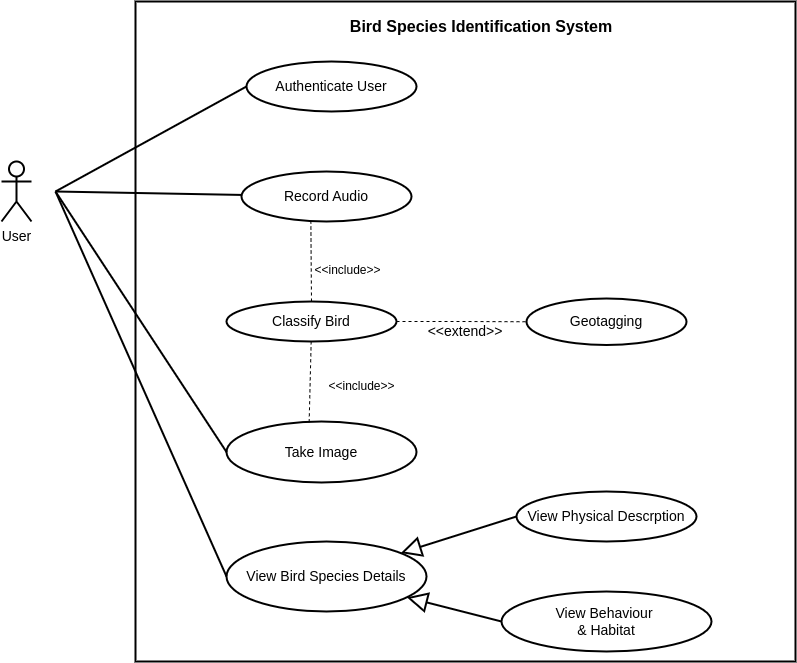
\includegraphics[scale=0.5]{images/usecase.png}
    \caption{Usecase Diagram for
        FeatherFind}%\label{fig:fig1}
\end{figure}

% \begin{figure}[h!]
%      \centering
%         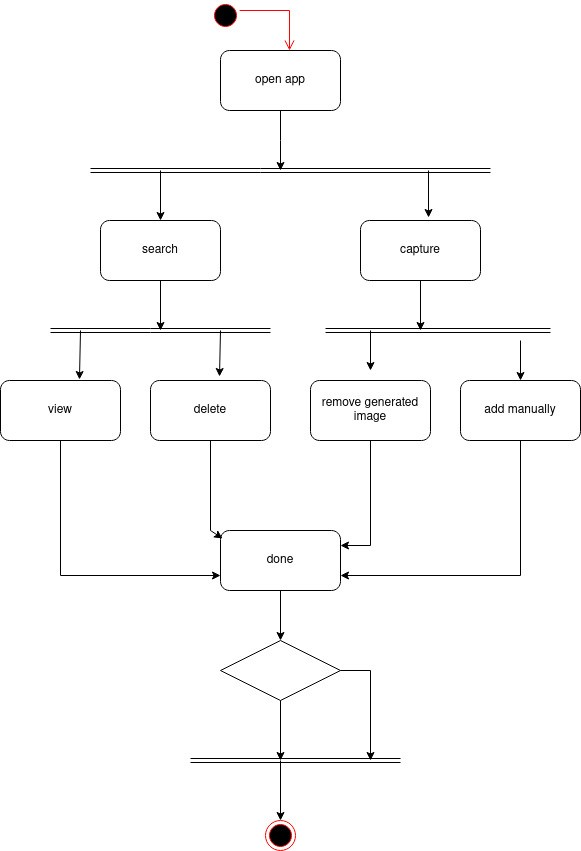
\includegraphics[scale=0.7]{output/activity.jpg}
%         \caption{Activity Diagram}%\label{fig:fig1}
%      \end{figure}
%      \newpage
% \newpage
\newpage
\section{Software Development Model}
This project will be using an incremental methodology since it offers a
functioning prototype at an early stage of development. The requirements and
scope of the project can be altered as necessary by studying the prototype. The
rationale for the preference for this software development strategy is the
flexibility offered by adopting the incremental technique. In this paradigm,
the project goes through several releases or iterations prior to its official
release.
\begin{figure}[h!]
    % \centering
    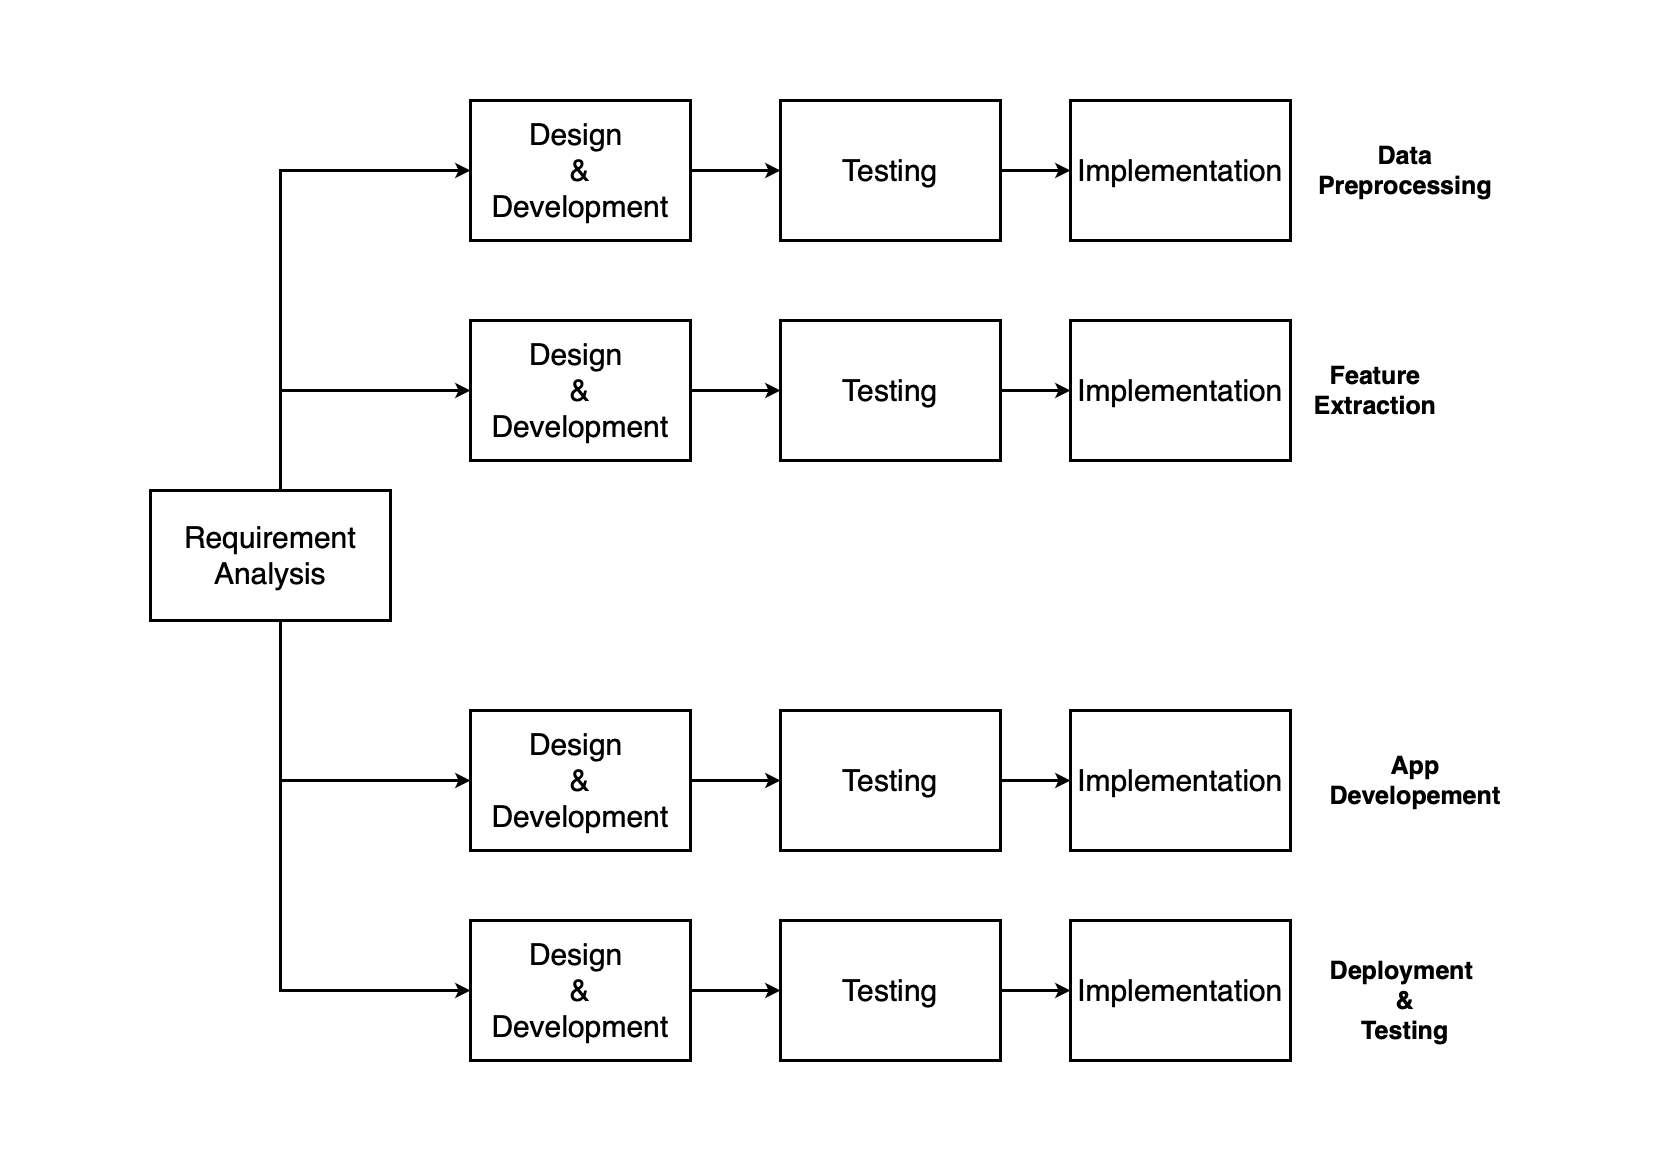
\includegraphics[scale=0.25]{images/SDLC.png}
    \caption{Incremental Model for development of
        FeatherFind}%\label{fig:fig1}
\end{figure}
\newpage

\chapter{Epilogue}
\section{Work Done}
In the course of our project on Bird Species Classification from Audio, we have accomplished several key tasks to progress our analysis and model development:

\subsection{Data Collection}
We curated a dataset of bird calls for 41 bird species found in Nepal using Xeno-Canto, a globally recognized repository of bird sound recordings. This platform provided diverse audio recordings for the selected bird species, forming the foundation of our dataset.
\begin{figure}[h!]
    \centering
    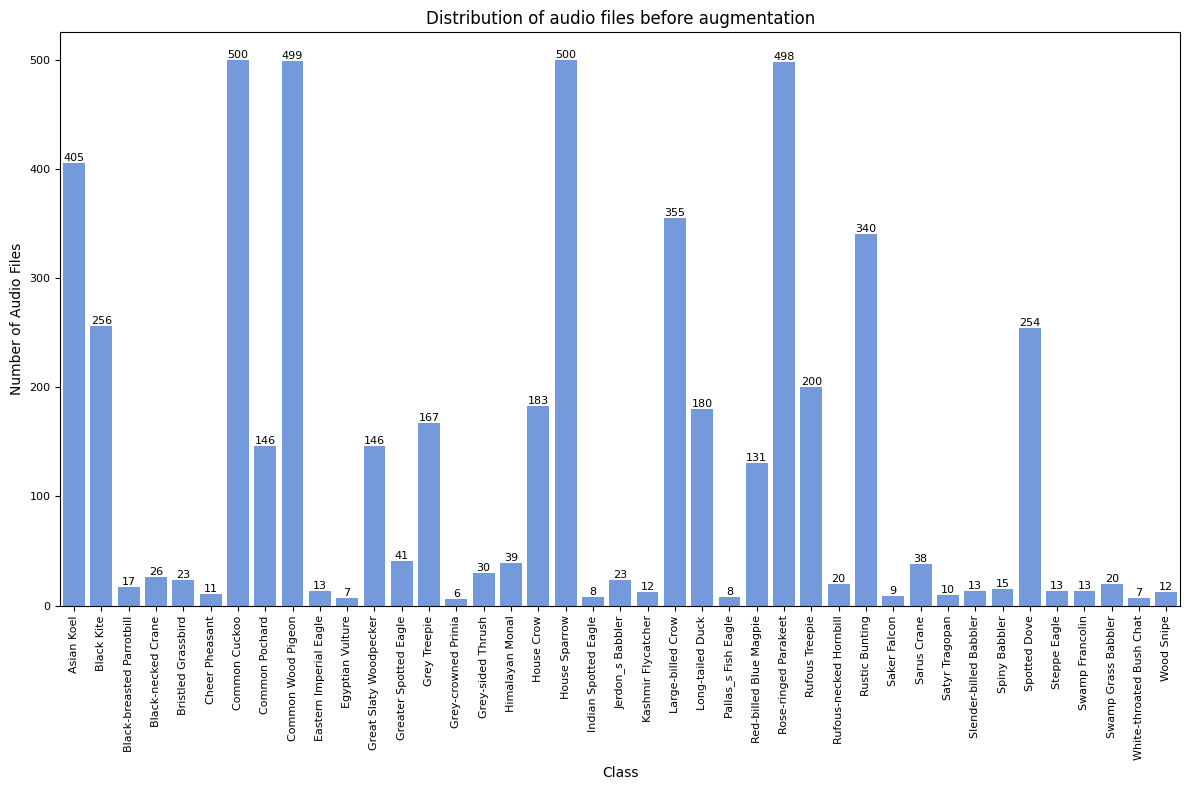
\includegraphics[width=0.8\textwidth]{images/before_augmentation.png}
    \caption{Data before performing augmentation}
    \label{fig:visualization}
\end{figure}

\newpage
\subsection{Data Augmentation}
Initial analysis of the collected data revealed significant class imbalance, with some species having over 400 recordings while others had fewer than 50. Additionally, the audio recordings varied in length. To address these issues:  
\begin{itemize}
    \item \textbf{Audio Clipping:}  
    \begin{itemize}
        \item Recordings were clipped into segments of 10 seconds each.  
        \item Clips shorter than 5 seconds were discarded to avoid blank audio segments and insufficient data.  
        \item Clips between 5 and 10 seconds were padded with silence at the end to standardize their length to 10 seconds.  
    \end{itemize}

    \item \textbf{Augmentation Techniques:}  
    To balance the dataset, augmentation techniques such as time stretching, phase shifting, and noise addition were applied. The parameters were varied to ensure diversity in the augmented data.  
    \begin{itemize}
        \item Each bird class was augmented to contain exactly 500 audio clips.
    \end{itemize}
\end{itemize}

\begin{figure}[h!]
    \centering
    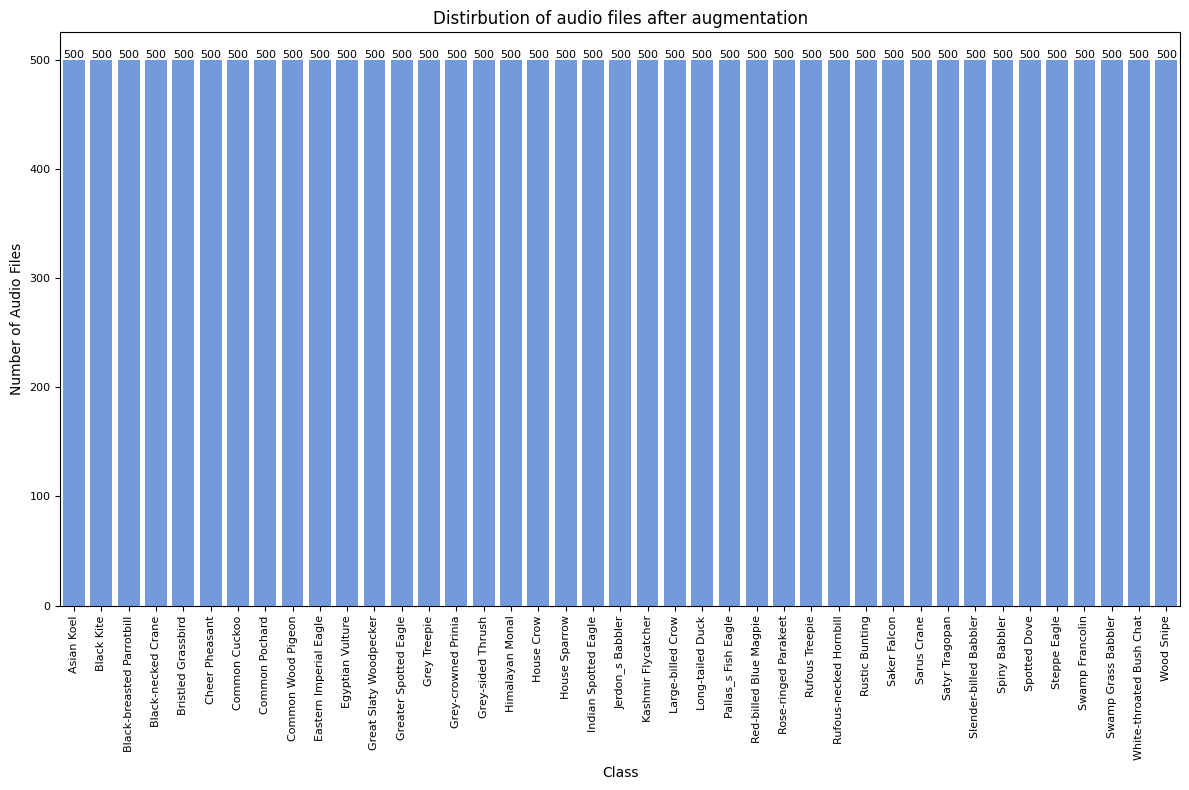
\includegraphics[width=0.8\textwidth]{images/after_augmentation.png}
    \caption{Data after performing augmentation}
    \label{fig:visualization}
\end{figure}



\newpage

\subsection{Data Preprocessing}
The audio recordings were transformed into Mel Spectrograms for further analysis.  

\begin{itemize}
    \item \textbf{Conversion Details:}  
    \begin{itemize}
        \item Audio files were converted using a sample rate of 32,000 Hz.  
        \item The spectrograms were generated with a Hanning window and 48 Mel bands.  
    \end{itemize}

    \item \textbf{Dataset Expansion:}  
    \begin{itemize}
        \item Each of the 500 audio files per bird class was converted into corresponding Mel Spectrogram images.  
        \item The resulting dataset was divided into training, validation, and testing sets for model development.
    \end{itemize}
\end{itemize}

\subsection{Model Training}  
The classification model was built using \textbf{EfficientNetB3} as the base architecture.  

\begin{itemize}
    \item \textbf{Input Preprocessing:}  
    \begin{itemize}
        \item Mel Spectrogram images were resized to \(128 \times 128 \times 3\) and normalized using the preprocess\_input function of EfficientNet.  
    \end{itemize}

    \item \textbf{Regularization:}  
    \begin{itemize}
        \item Dropout layers and kernel regularizers were employed to mitigate overfitting.  
    \end{itemize}

    \item \textbf{Callback Functions:}  
    \begin{itemize}
        \item Early stopping, learning rate reduction on plateau, and checkpoint saving mechanisms were implemented to enhance training efficiency and performance.  
    \end{itemize}

    \item \textbf{Performance:}  
    \begin{itemize}
        \item On the test set, the model achieved an accuracy of \textbf{89.36\%} with a cross-entropy loss of \textbf{0.42}.  
    \end{itemize}
\end{itemize}

\subsection{Genetic Algorithm for Hyperparameter Tuning}
To optimize the performance of our model, we used genetic algorithm for hyperparameter tuning. 
This approach helped us systematically explore and identify the most effective hyperparameter settings for our model, 
including learning rates, batch sizes, and network architecture parameters. 
The genetic algorithm enabled a more efficient and comprehensive search for optimal configurations.


\begin{figure}[h!]
    \centering
    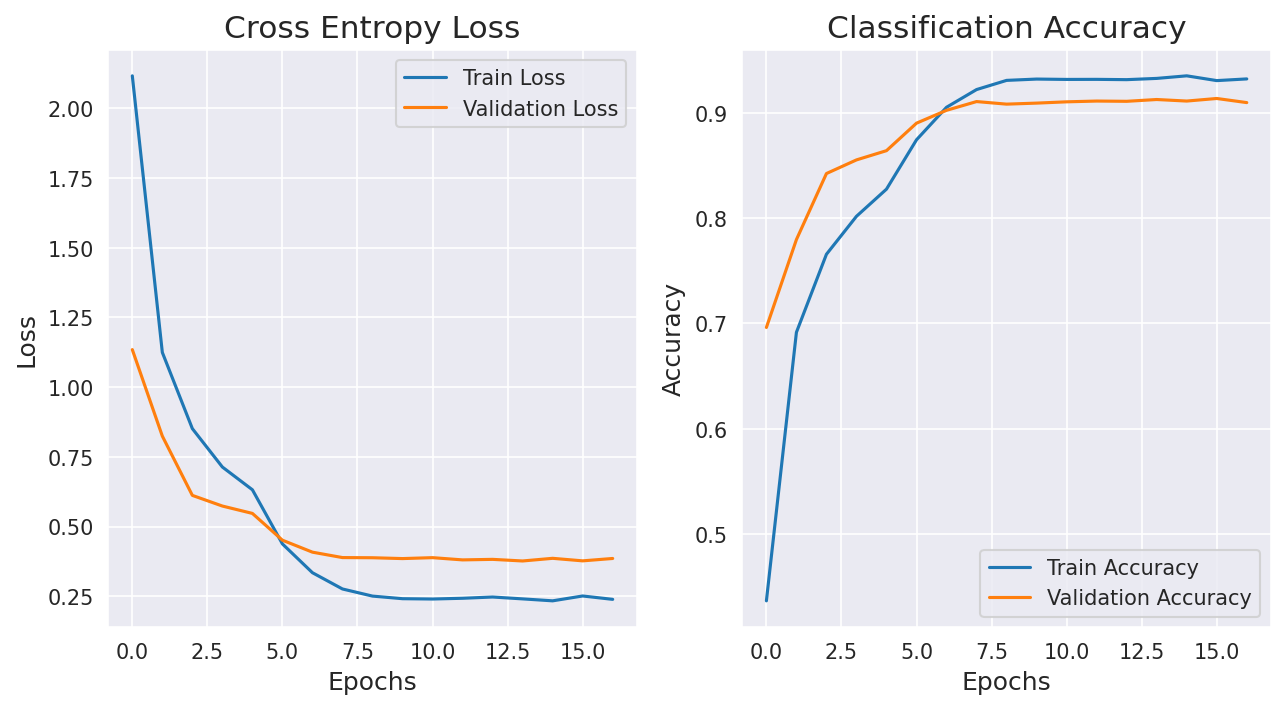
\includegraphics[width=0.8\textwidth]{images/accuracy_and_loss.png}
    \caption{Accuracy and Cross-entropy loss for train and validation sets}
    \label{fig:visualization}
\end{figure}

\begin{figure}[h!]
    \centering
    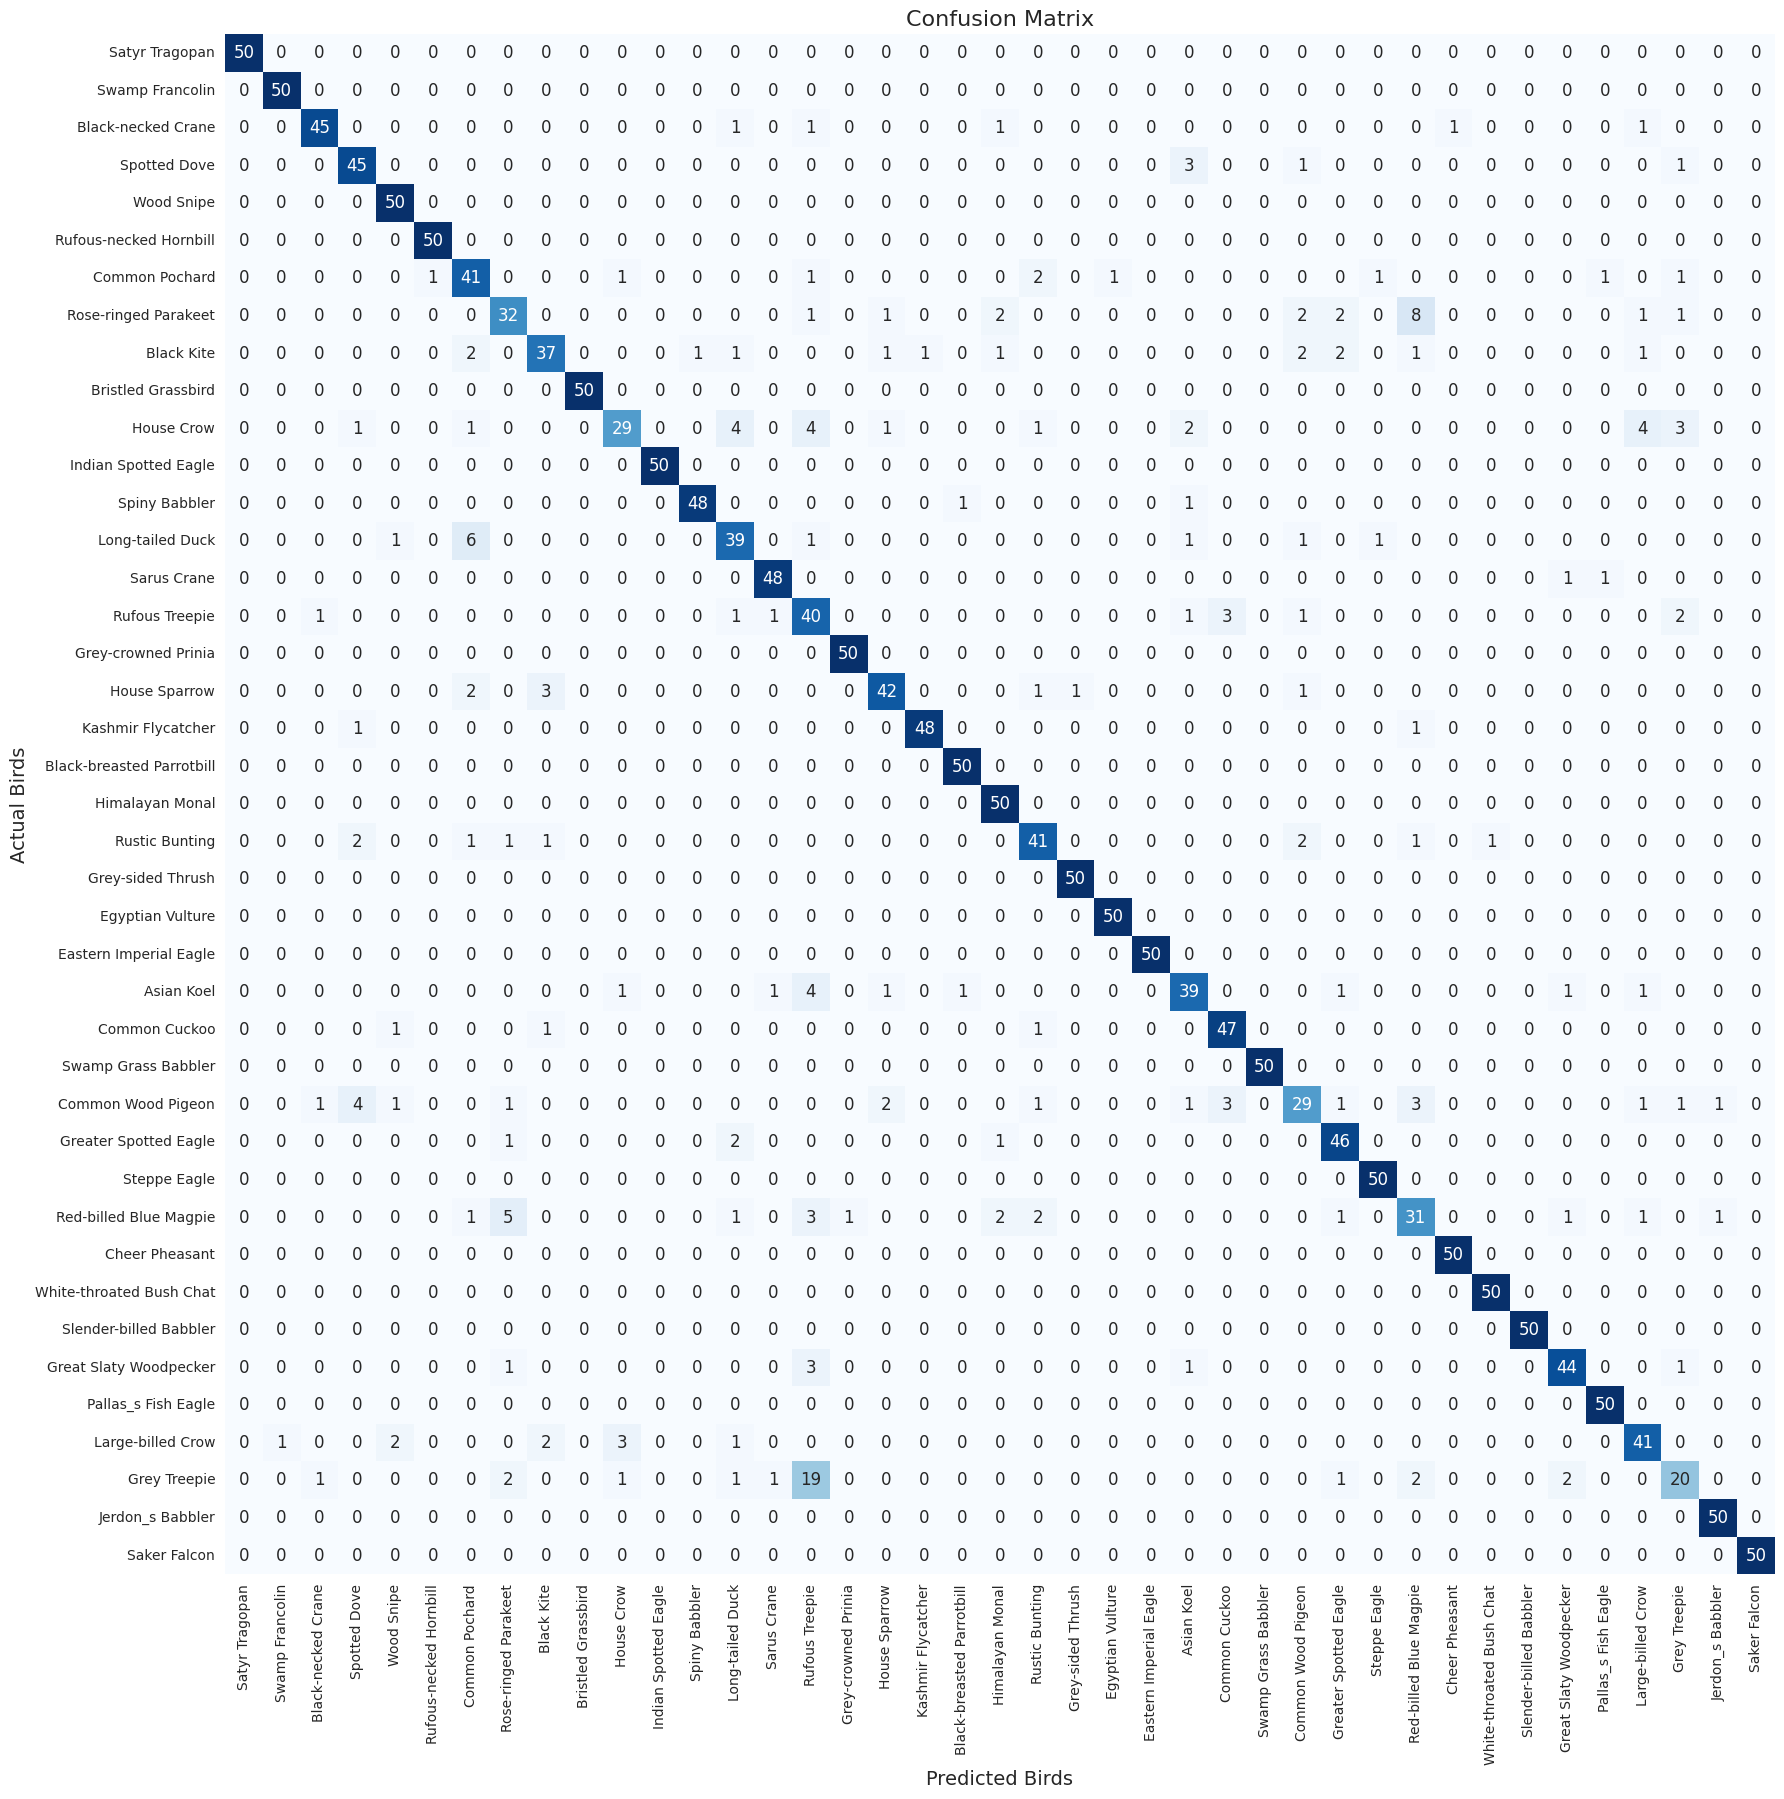
\includegraphics[scale=0.3]{images/confusion_matrix.png}
    \caption{Confusion matrix for the model on test set.}
    \label{fig:Confusion matrix}
\end{figure}

\begin{figure}[h!]
    \centering
    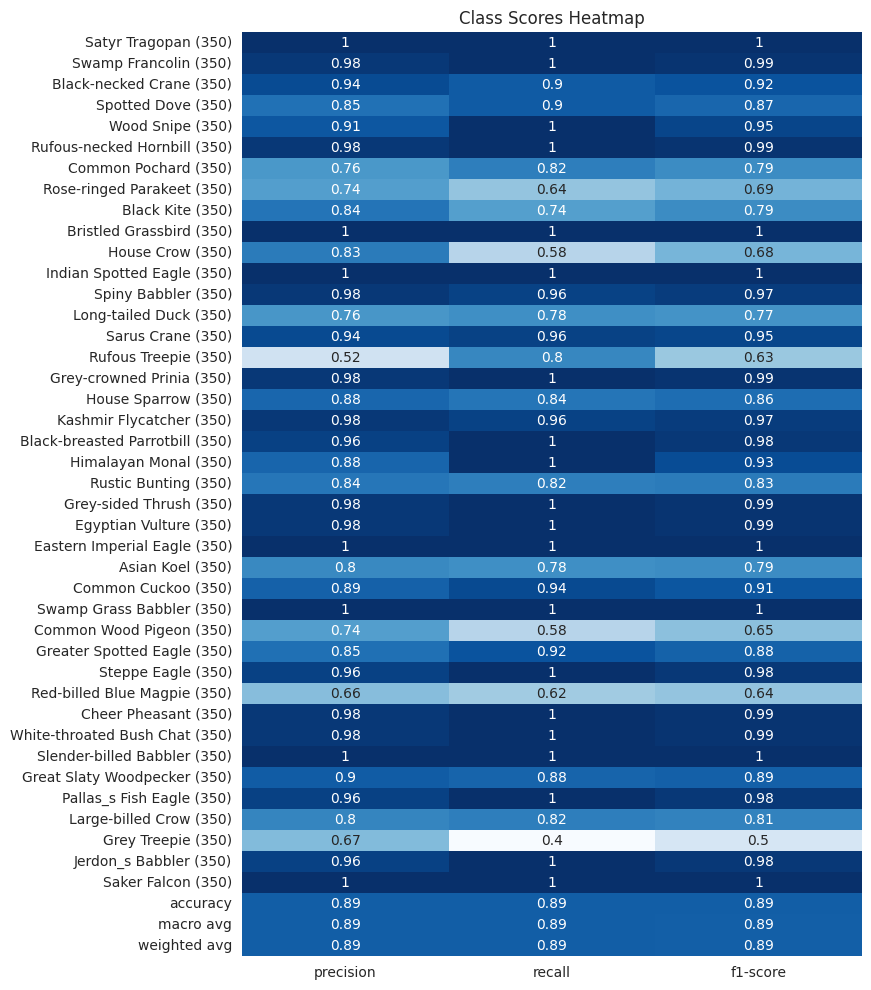
\includegraphics[scale=0.45]{images/classification_report.png}
    \caption{Classification report of the model.}
    \label{fig:Classification report}
\end{figure}

\newpage
\subsection{Deployment to Huggingface spaces}
A FastAPI application was developed using the trained model and deployed on \textbf{Huggingface spaces}. This deployment enables seamless API integration, allowing users to interact with the model for predictions efficiently and reliably.


\subsection{Bird Sound Detection Model Training}

To enhance the reliability of the species classification system, we incorporated a Bird Sound Detection model as a preliminary step to verify the presence of bird sounds in recorded audio. This approach is inspired by Lasseck (2018) \cite{lasseck2018acoustic}, which demonstrated the effectiveness of using Deep Convolutional Neural Networks (DCNNs) for acoustic bird detection, achieving an AUC score exceeding \textbf{93.7\%} on unseen data. Following this methodology, we employed a pre-trained InceptionV3 network for our binary classification task, achieving an initial AUC score of \textbf{83\%}.

Dataset used for the training of the Bird Sound Detection Model is Field recordings, worldwide ("freefield1010") - a collection of 7,690 excerpts from field recordings around the world, gathered by the FreeSound project, and then standardised for research. This collection is very diverse in location and environment, and for the BAD Challenge we have annotated it for the presence/absence of birds.
% Image for Bird Sound Detection Model Training
\begin{figure}[h!]
    \centering
    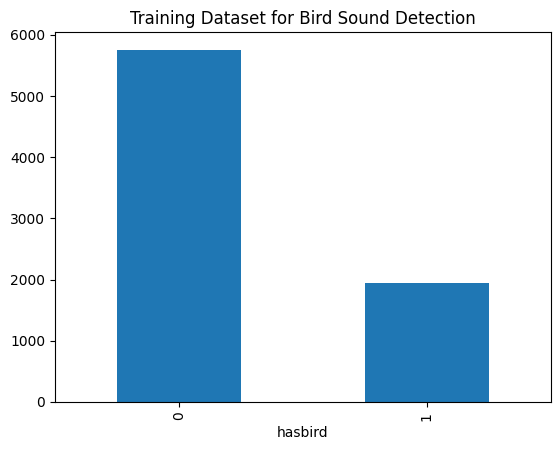
\includegraphics[scale=0.45]{images/det_trainingdataset.png}
    \caption{Dataset distribution for freefield1010}
    \label{fig:freefield1010 dataset}
\end{figure}


Dataset used for the evaluating the model's performance is Crowdsourced dataset, UK ("warblrb10k") - 8,000 smartphone audio recordings from around the UK, crowdsourced by users of Warblr the bird recognition app. The audio covers a wide distribution of UK locations and environments, and includes weather noise, traffic noise, human speech and even human bird imitations.
\begin{figure}[h!]
    \centering
    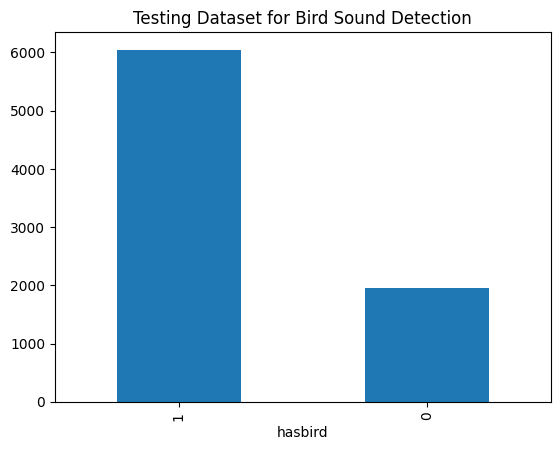
\includegraphics[scale=0.45]{images/det_testingdataset.png}
    \caption{Dataset distribution for warblrb10k}
    \label{fig:warblrb10k dataset}
\end{figure}
\newpage
After the model was subjected to the testing dataset, the following confusion matrix was obtained, yielding an accuracy of \textbf{87.28\%}.
\begin{figure}[h!]
    \centering
    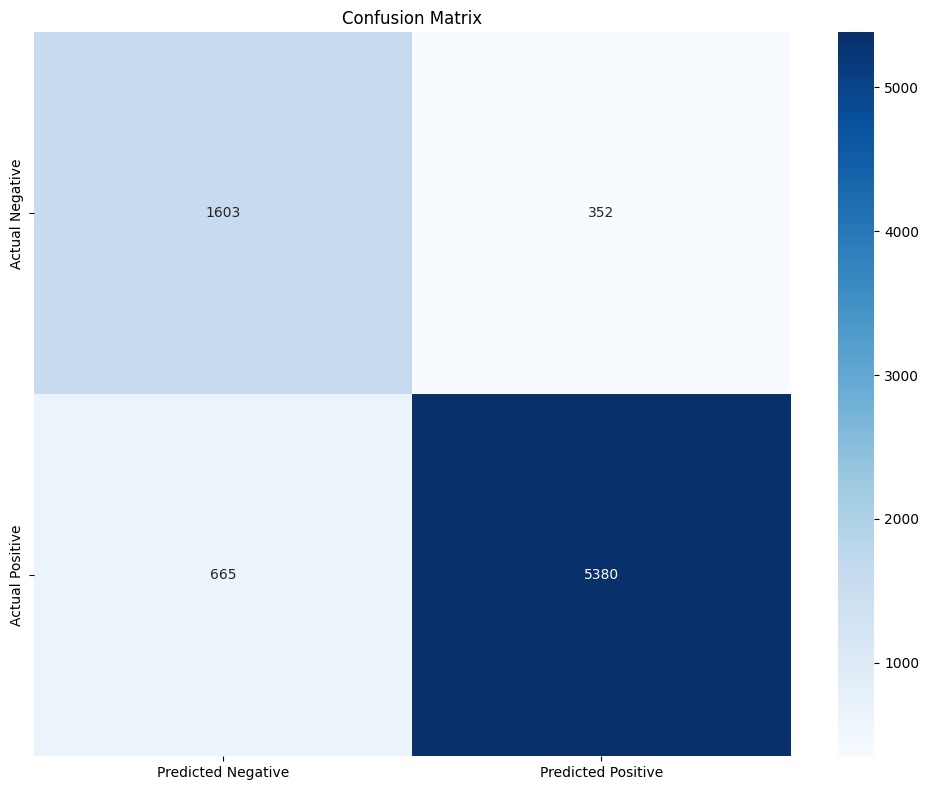
\includegraphics[scale=0.35]{images/det_confusionmatrix.png}
    \caption{Confusion Matrix for Bird Sound Detection Model}
    \label{fig:Confusion Matrix for Detection Model}
\end{figure}

To assess the effectiveness of our model in distinguishing between the target classes, we analyzed its performance using the Receiver Operating Characteristic (ROC) curve. The ROC curve provides a comprehensive view of the trade-off between the true positive rate (TPR) and the false positive rate (FPR) at various threshold settings. The Area Under the Curve (AUC) metric, derived from the ROC curve, quantifies the overall discriminatory power of the model, with a higher AUC indicating better performance.
\begin{figure}[h!]
    \centering
    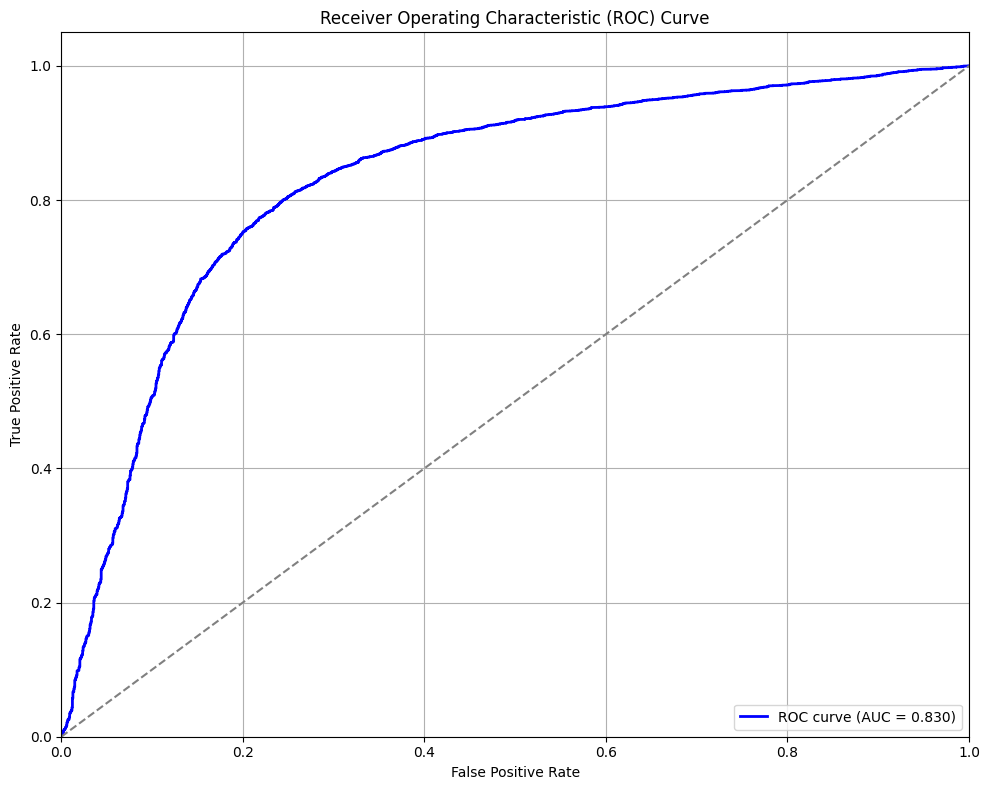
\includegraphics[scale=0.35]{images/det_roc.png}
    \caption{ROC Curve of the detection model}
    \label{fig:ROC Curve}
\end{figure}

While our results are promising and validate the model's applicability, the specific preprocessing and data augmentation techniques outlined in the reference study, such as time and frequency stretching and the use of a high-pass filter, were not implemented. Incorporating these methods in future iterations could further enhance the model's performance and generalization to diverse recording conditions.

\newpage


% Include image for model training
\newpage

\subsection{Mobile App Development}
The mobile application allows the user to record the audio, visualize it with waveforms during recording, 
before sending the actual audio data to the server for processing. The user can also use the application to 
add their current location to the map. 

\begin{figure}[h!]
    \centering
    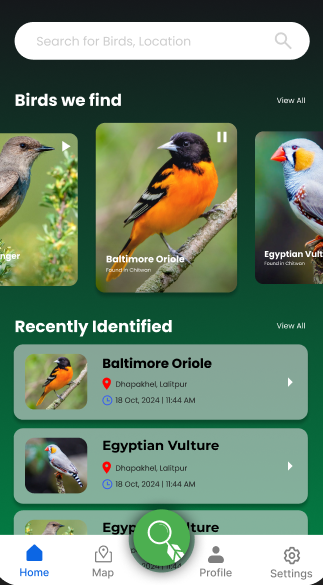
\includegraphics[scale=0.5]{images/homepage.png}
    \caption{Home Page of FeatherFind.}
\end{figure}

\begin{figure}[h!]
    \centering
    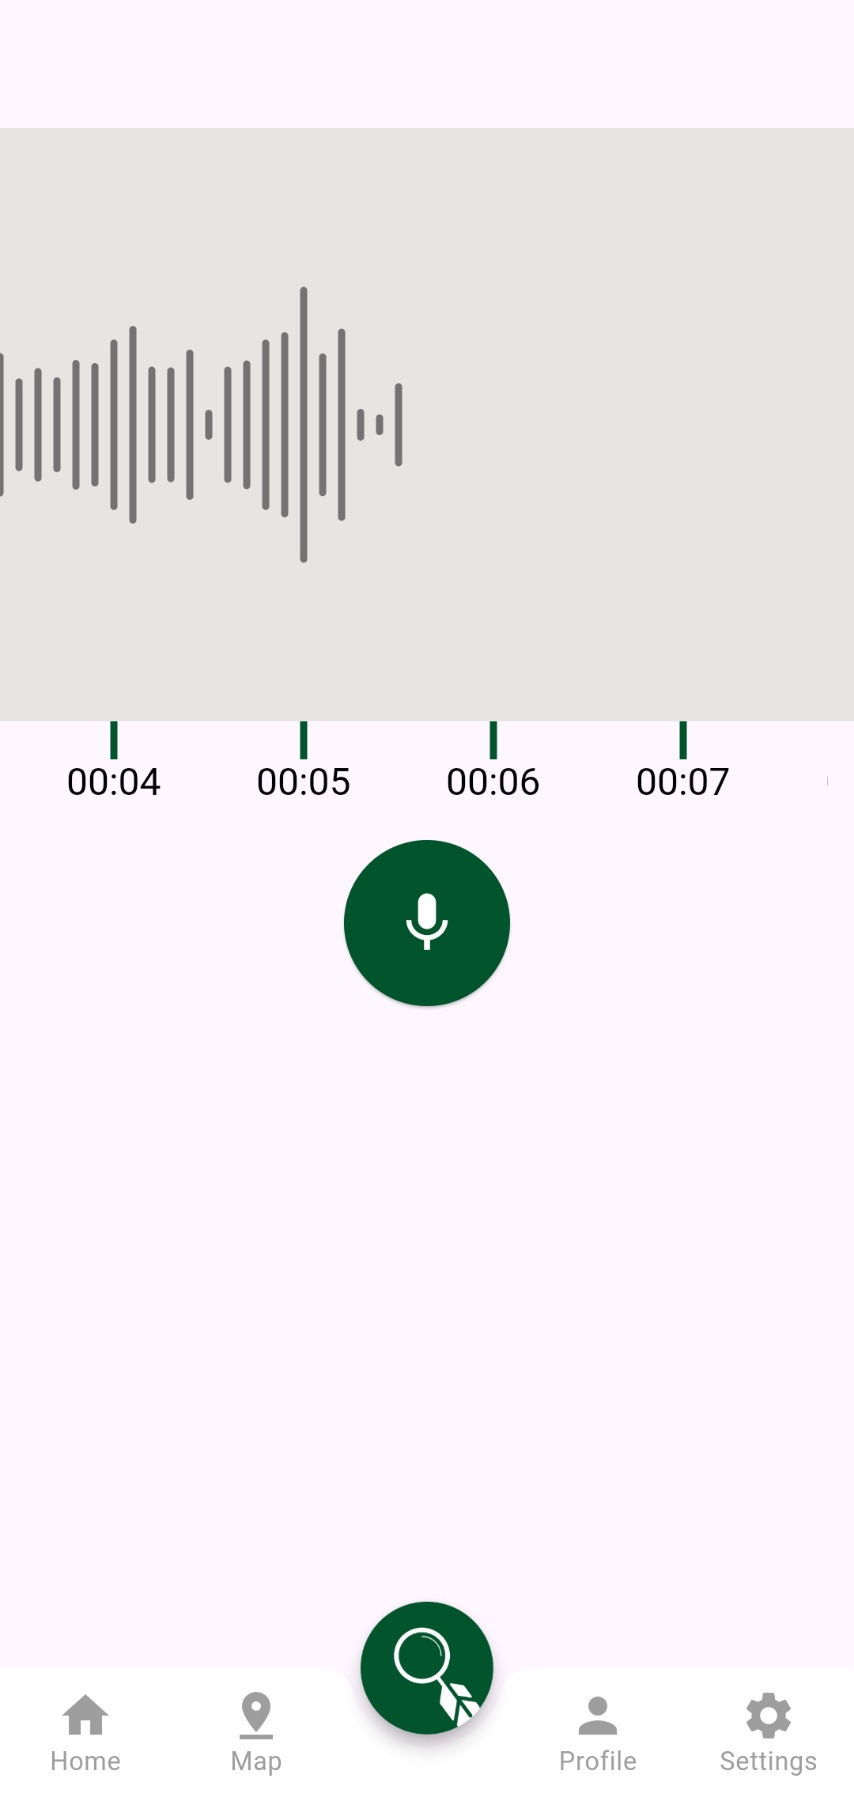
\includegraphics[scale=0.18]{images/Recordingpage.jpg}
    \caption{Audio Recording using FeatherFind.}
\end{figure}

\newpage


\section{Work Remaining}
While substantial progress has been made in the Bird Species Classification
from Audio project, several critical tasks remain to be addressed to further refine and enhance the system:

% \subsection{Improved Data Augmentation}
% To address potential imbalances in the dataset and improve model performance,
%  we will implement advanced data augmentation techniques. This involves creating 
%  additional variations of the audio files through methods such as pitch shifting, 
%  time stretching, and adding synthetic noise. Enhanced data augmentation will help 
%  balance the dataset and provide a more diverse range of examples for the model to learn from.

% \subsection{Model Training with CNN+LSTM}
% We will extend our model training to include a hybrid Convolutional Neural Network (CNN) and Long Short-Term Memory (LSTM) network. The combination of CNNs and LSTMs is expected to capture both spatial and temporal features in the audio data more effectively, potentially leading to improved classification accuracy. We will experiment with various architectures and configurations to identify the most effective setup for our classification task.

\subsection{Genetic Algorithm for Hyperparameter Tuning}
To optimize the performance of our model, we used genetic algorithm for hyperparameter tuning. This approach helped us systematically explore and identify the most effective hyperparameter settings for our model, including learning rates, batch sizes, and network architecture parameters. The genetic algorithm enabled a more efficient and comprehensive search for optimal configurations.

\subsection{Mobile App Integration}
Once the model is properly trained and optimized, the next step will be to integrate the machine learning model into a mobile application. The mobile app will capture audio input from the user, preprocess it (e.g., feature extraction), and then feed it into the deployed model for classification.

These remaining tasks are essential to advancing the project and achieving our goal of an accurate and reliable bird species classification system from audio data. 

\newpage

%Reference
\renewcommand\bibname{REFERENCES} % Change heading to References
\bibliographystyle{IEEEtran} % to use IEEE Format for referencing
\addcontentsline{toc}{chapter}{References} % to add references in TOC
\bibliography{library} % specify the .bib file containing reference information 

%Comment this Chapter if you do not need to include Appendix.

%\addcontentsline{toc}{chapter}{Appendix}


\end{document}
